 \documentclass[12pt]{article}
\usepackage[utf8]{inputenc}
\usepackage{amsmath}
\usepackage{amssymb}
\usepackage[english]{babel}
\usepackage[margin = 1 in]{geometry}
\usepackage{wrapfig}
\usepackage{enumitem}
\usepackage{caption}
\usepackage{csquotes}
\usepackage{xcolor}
\usepackage{graphicx} 
\usepackage{subfig}

\usepackage{subfig}

\title{Project 2 - SI1336 Simulation and modelling}
\author{Raymond Wang} 
\date{November 18, 2020}
\begin{document}
\maketitle
\newpage
\section*{Project 2.1}
\subsection*{2.1a) Two-dimensional random walks with 10-100 steps}
\begin{figure*}[ht!]
\begin{center}
   \subfloat[\label{genworkflow}]{%
      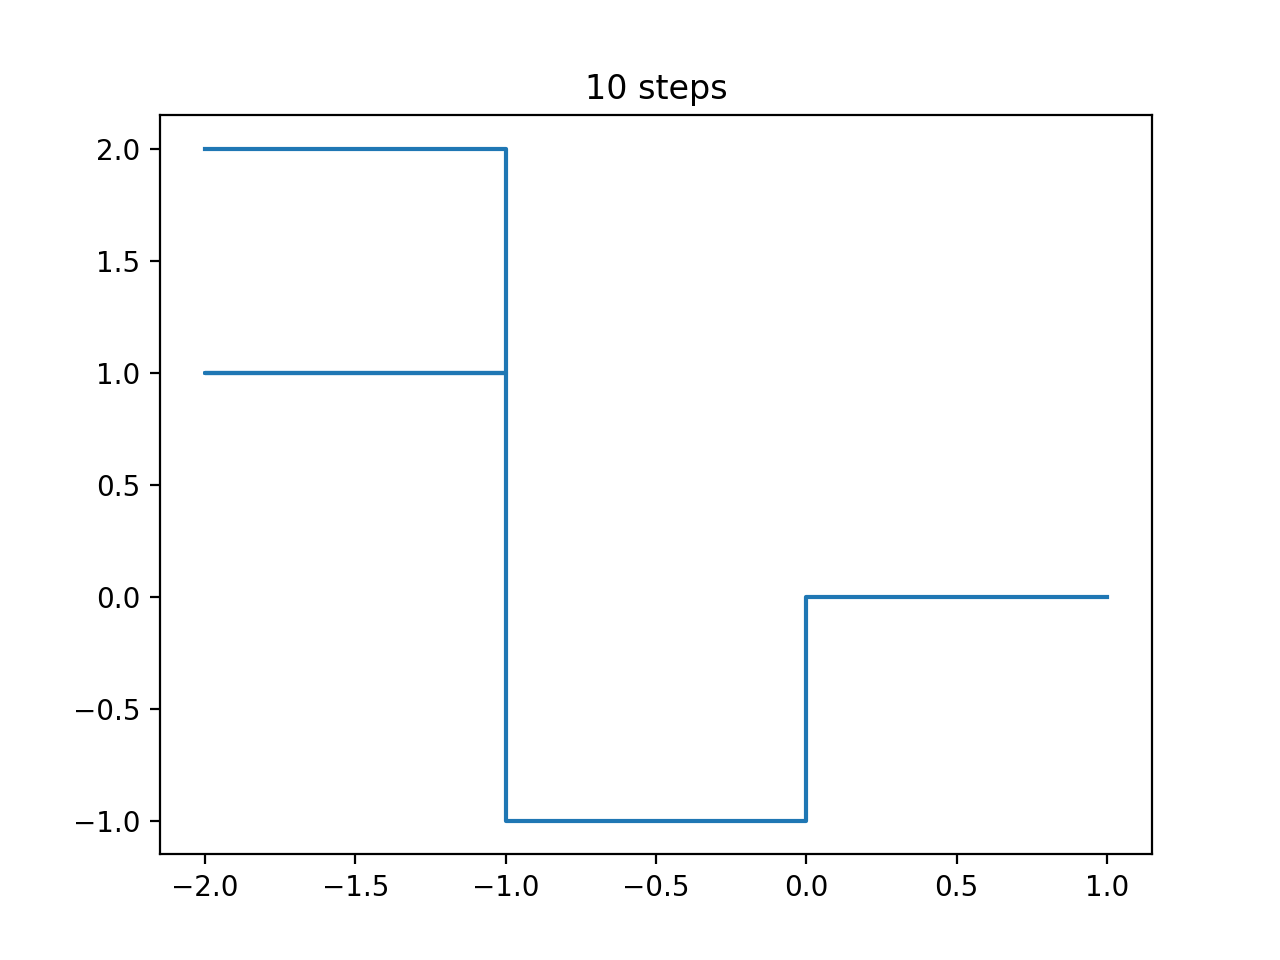
\includegraphics[width=0.33\textwidth]{10_steps.jpg}}
   \subfloat[\label{pyramidprocess}]{%
      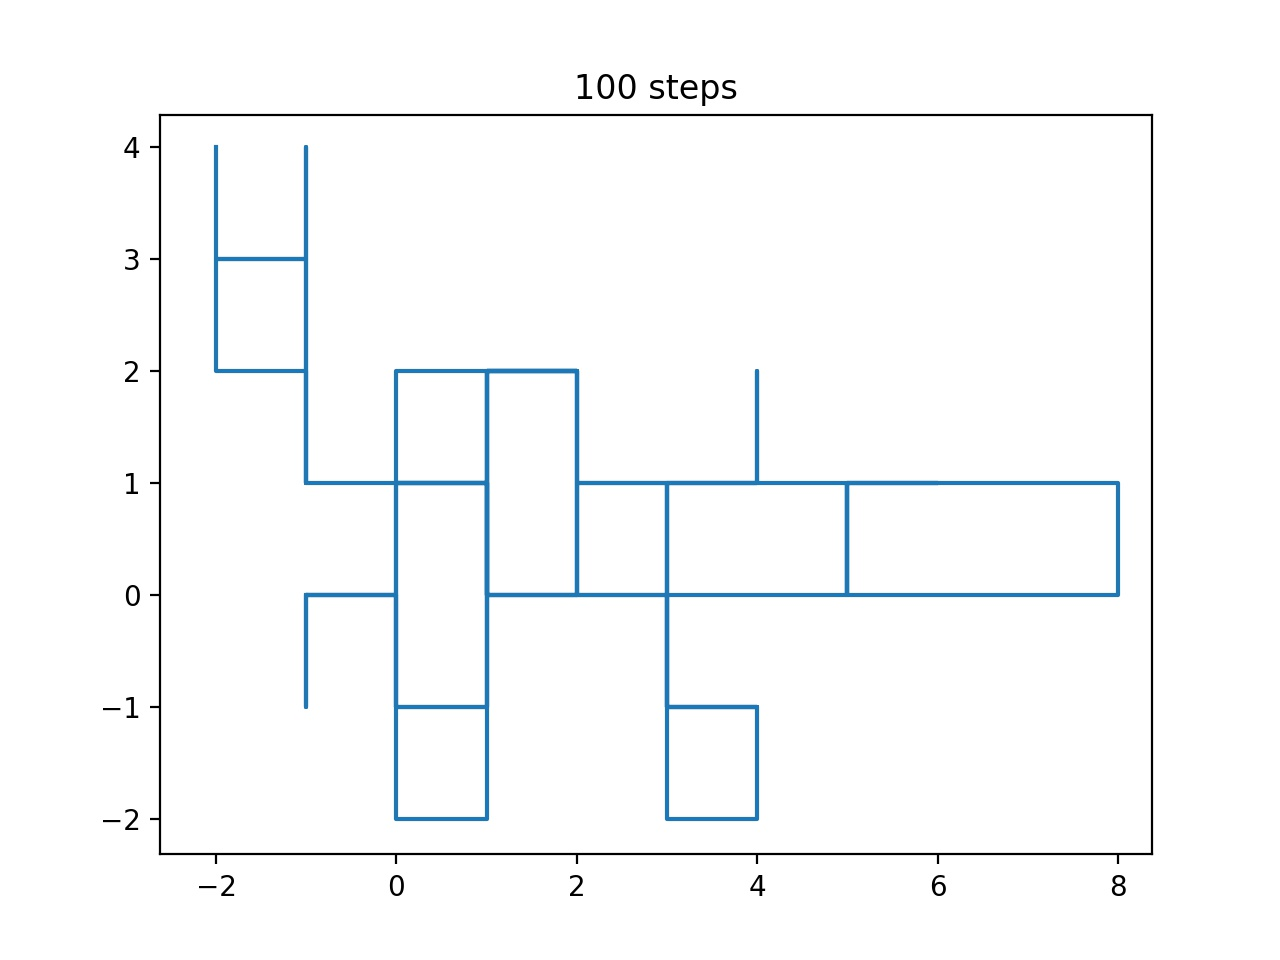
\includegraphics[ width=0.33\textwidth]{100_steps.jpg}}
   \subfloat[\label{mt-simtask}]{%
      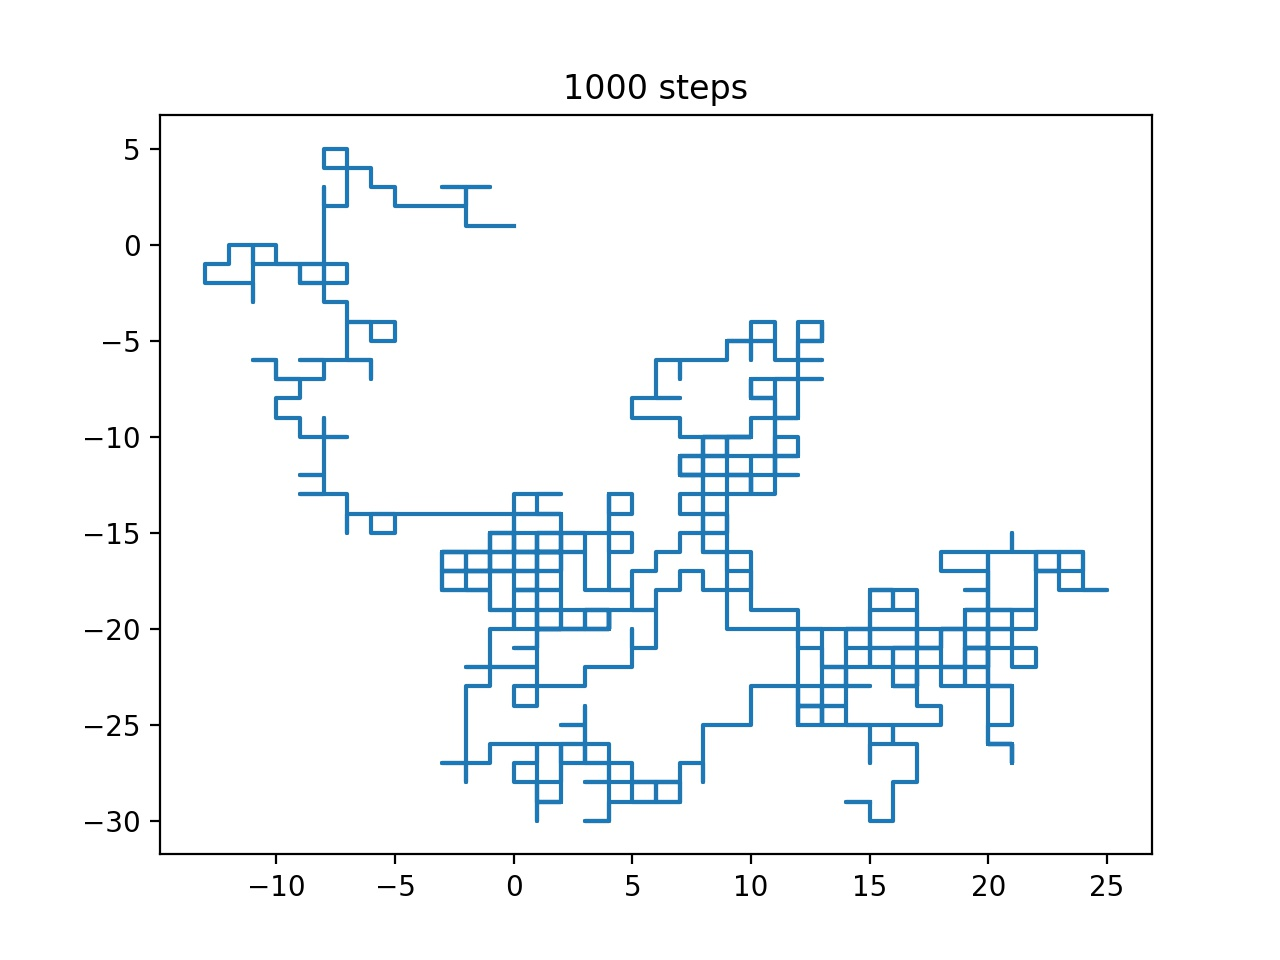
\includegraphics[ width=0.33\textwidth]{1000_steps.jpg}}\\
   \caption{\label{workflow} (a) 10 steps (b) 100 steps; (c) 1000 steps}
\end{center}
\end{figure*}
\noindent 
Evidently, the walk paths become more complex and randomized as the number of steps increases.

\subsection*{2.1b) Random walks for customized random generator}
Utilizing a random generator $r_n = (a r_{n-1} + c) \bmod m $ with step size 1000, setting parameters

\begin{equation*}
r_0 = 1,\quad a = 3, \quad c = 4,
\end{equation*}
and varying $m$, the following walks are generated:

\begin{figure*}[ht!]
\begin{center}
   \subfloat[\label{genworkflow}]{%
      \includegraphics[width=0.33\textwidth]{randomwalk_1000_r{1}_a{3}_c{4}_m{128}.jpg}}
   \subfloat[\label{pyramidprocess}]{%
      \includegraphics[ width=0.33\textwidth]{randomwalk_1000_r{1}_a{3}_c{4}_m{129}.jpg}}
   \subfloat[\label{mt-simtask}]{%
      \includegraphics[ width=0.33\textwidth]{randomwalk_1000_r{1}_a{3}_c{4}_m{130}.jpg}}\\
   \caption{\label{workflow} (a) $m = 128$ (b) $m = 129$ (c) $m = 130$}
\end{center}
\end{figure*}
\noindent By varying the remaining parameters, differing walks are to be observed, except for $r_0$.

\begin{figure*}[ht!]
\textbf{Dependence on r (a = 3, c = 4, m = 128)}
\begin{center}
   \subfloat[\label{genworkflow}]{%
      \includegraphics[width=0.33\textwidth]{randomwalk_1000_r{1}_a{3}_c{4}_m{128}.jpg}}
   \subfloat[\label{pyramidprocess}]{%
      \includegraphics[ width=0.33\textwidth]{randomwalk_1000_r{2}_a{3}_c{4}_m{128}.jpg}}
   \subfloat[\label{mt-simtask}]{%
      \includegraphics[ width=0.33\textwidth]{randomwalk_1000_r{3}_a{3}_c{4}_m{128}.jpg}}\\
   \caption{\label{workflow} (a) $r_0 = 1$ (b) $r_0 = 2$ (c) $r_0 = 3$}
\end{center}
\end{figure*}


\begin{figure*}[ht!]
\textbf{Dependence on a (r = 1, c = 4, m = 128)}
\begin{center}
   \subfloat[\label{genworkflow}]{%
      \includegraphics[width=0.33\textwidth]{randomwalk_1000_r{1}_a{3}_c{4}_m{128}.jpg}}
   \subfloat[\label{pyramidprocess}]{%
      \includegraphics[ width=0.33\textwidth]{randomwalk_1000_r{1}_a{4}_c{4}_m{128}.jpg}}
   \subfloat[\label{mt-simtask}]{%
      \includegraphics[ width=0.33\textwidth]{randomwalk_1000_r{1}_a{5}_c{4}_m{128}.jpg}}\\
   \caption{\label{workflow} (a) $a = 3$ (b) $a = 4$ (c) $a =5$}
\end{center}
\end{figure*}

\begin{figure*}[ht!]
\textbf{Dependence on c (r = 1, a = 3, m = 128)}
\begin{center}
   \subfloat[\label{genworkflow}]{%
      \includegraphics[width=0.33\textwidth]{randomwalk_1000_r{1}_a{3}_c{4}_m{128}.jpg}}
   \subfloat[\label{pyramidprocess}]{%
      \includegraphics[ width=0.33\textwidth]{randomwalk_1000_r{1}_a{3}_c{5}_m{128}.jpg}}
   \subfloat[\label{mt-simtask}]{%
      \includegraphics[ width=0.33\textwidth]{randomwalk_1000_r{1}_a{3}_c{6}_m{128}.jpg}}\\
   \caption{\label{workflow} (a) $c = 4$ (b) $c = 5$ (c) $c =6$}
\end{center}
\end{figure*}

\newpage
\subsection*{2.1c) Comparisons for random walks with 1-1000 steps}

\begin{figure*}[ht!]
\begin{center}
    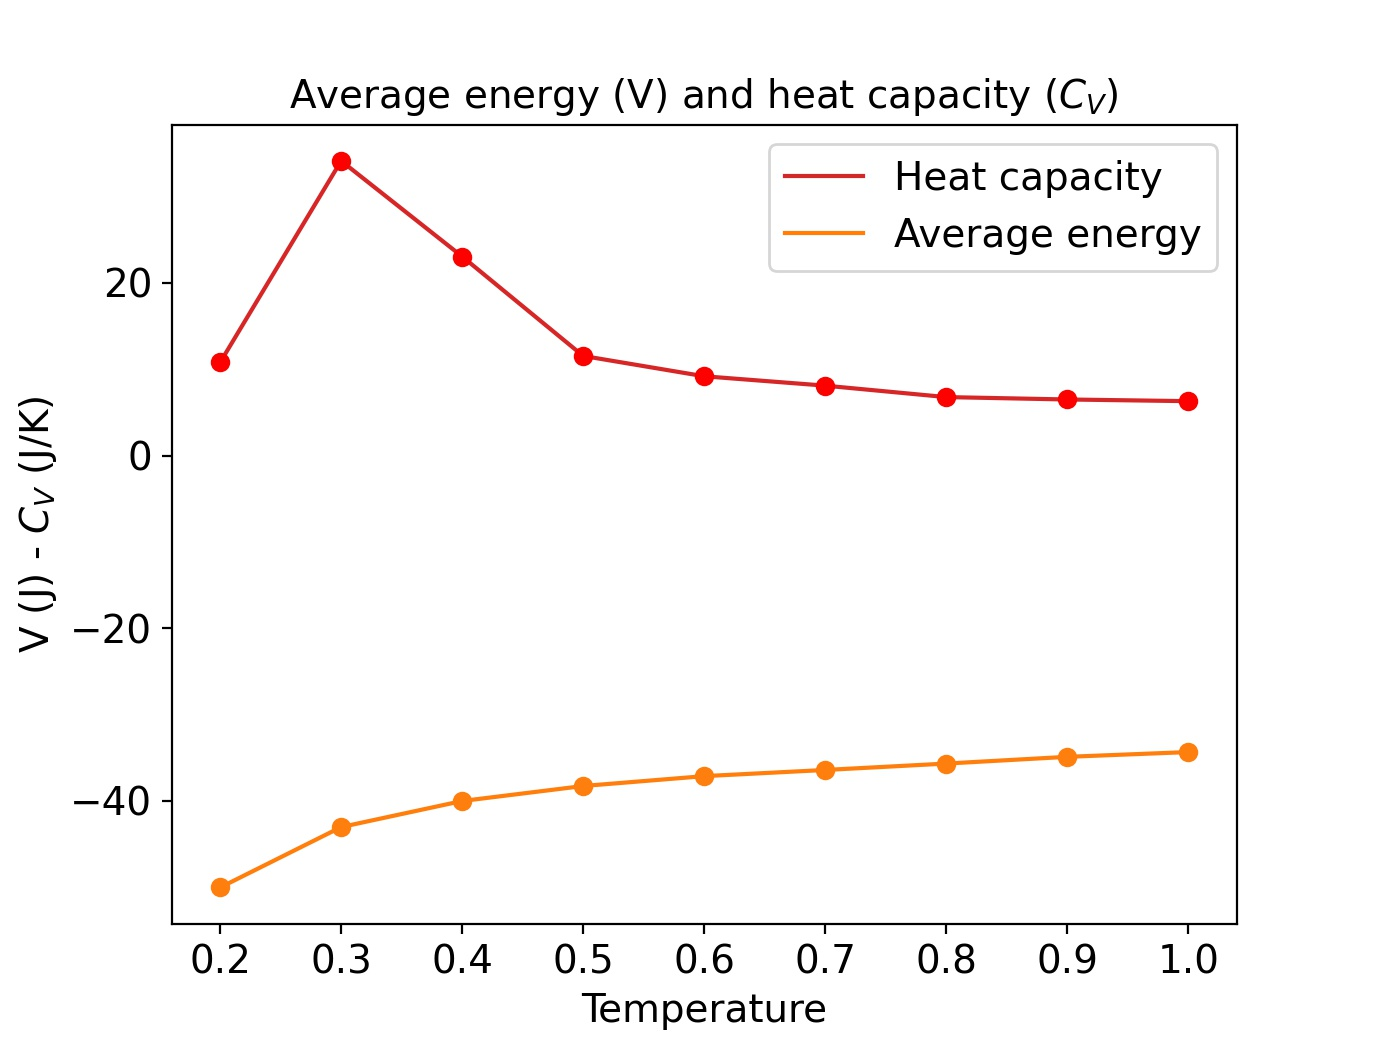
\includegraphics[width=0.5\textwidth]{Comparison.jpg}
 \caption{}
\end{center}
\end{figure*}

\noindent In the aforementioned diagram, the root mean squared end-to-end distance ($\sqrt{\langle R^2 \rangle})$, standard error estimate (STDE) and root-mean-square fluctuation (RMSF) are plotted against the the number of steps (N). As can be noted the, the correlation between N with RMSF and
($\sqrt{\langle R^2 \rangle}$) follow a typical square root relation, which indicates that the length ($\langle R^2 \rangle$) depends on N linearly.

\begin{figure*}[ht!]
\begin{center}
   \subfloat[\label{genworkflow}]{%
      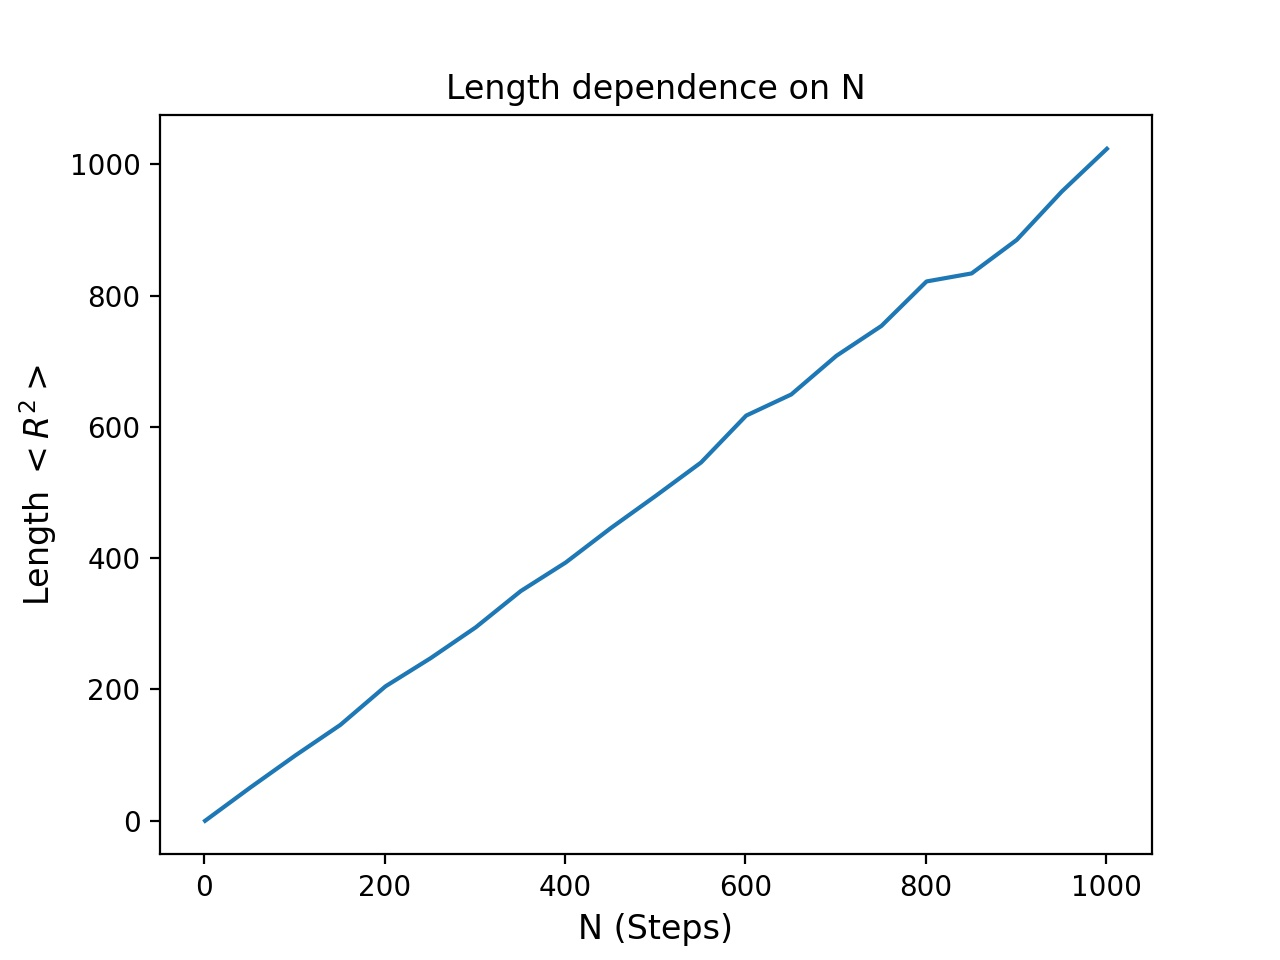
\includegraphics[width=0.45\textwidth]{MSD.jpg}}
   \subfloat[\label{pyramidprocess}]{%
      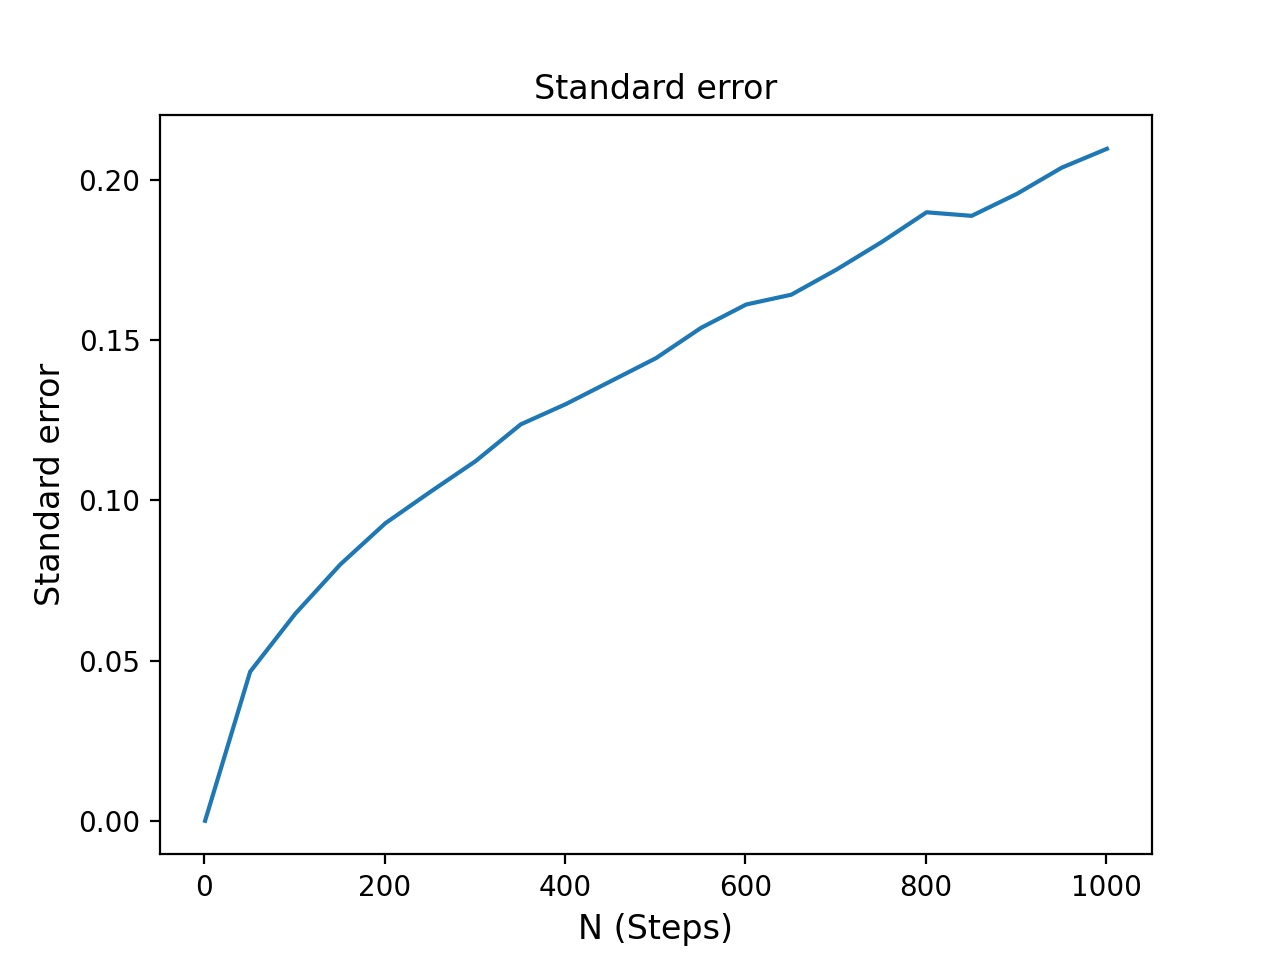
\includegraphics[ width=0.45\textwidth]{SEM.jpg}}\\
   \caption{\label{workflow} (a) Length dependence on N (b) Standard error}
\end{center}
\end{figure*}
\noindent As can be noted the Standard error is minuscule but correlating with N in the same manner as the other variables.

\newpage
\subsection*{2.1d) Non-intersecting random-walks}
\subsubsection*{Generated random walks}
\begin{figure*}[ht!]
\begin{center}
   \subfloat[\label{genworkflow}]{%
      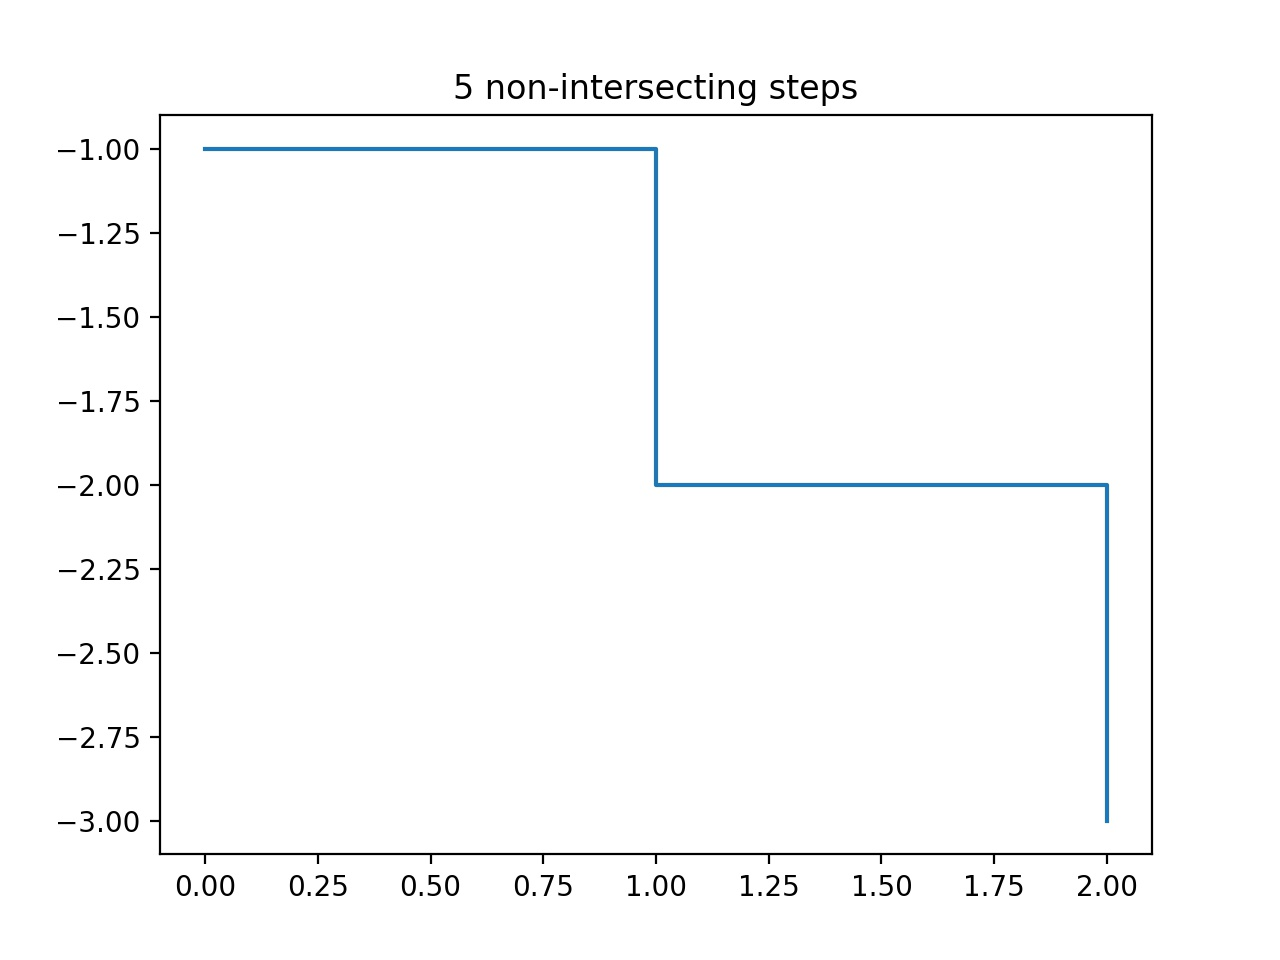
\includegraphics[width=0.33\textwidth]{5.jpg}}
   \subfloat[\label{pyramidprocess}]{%
      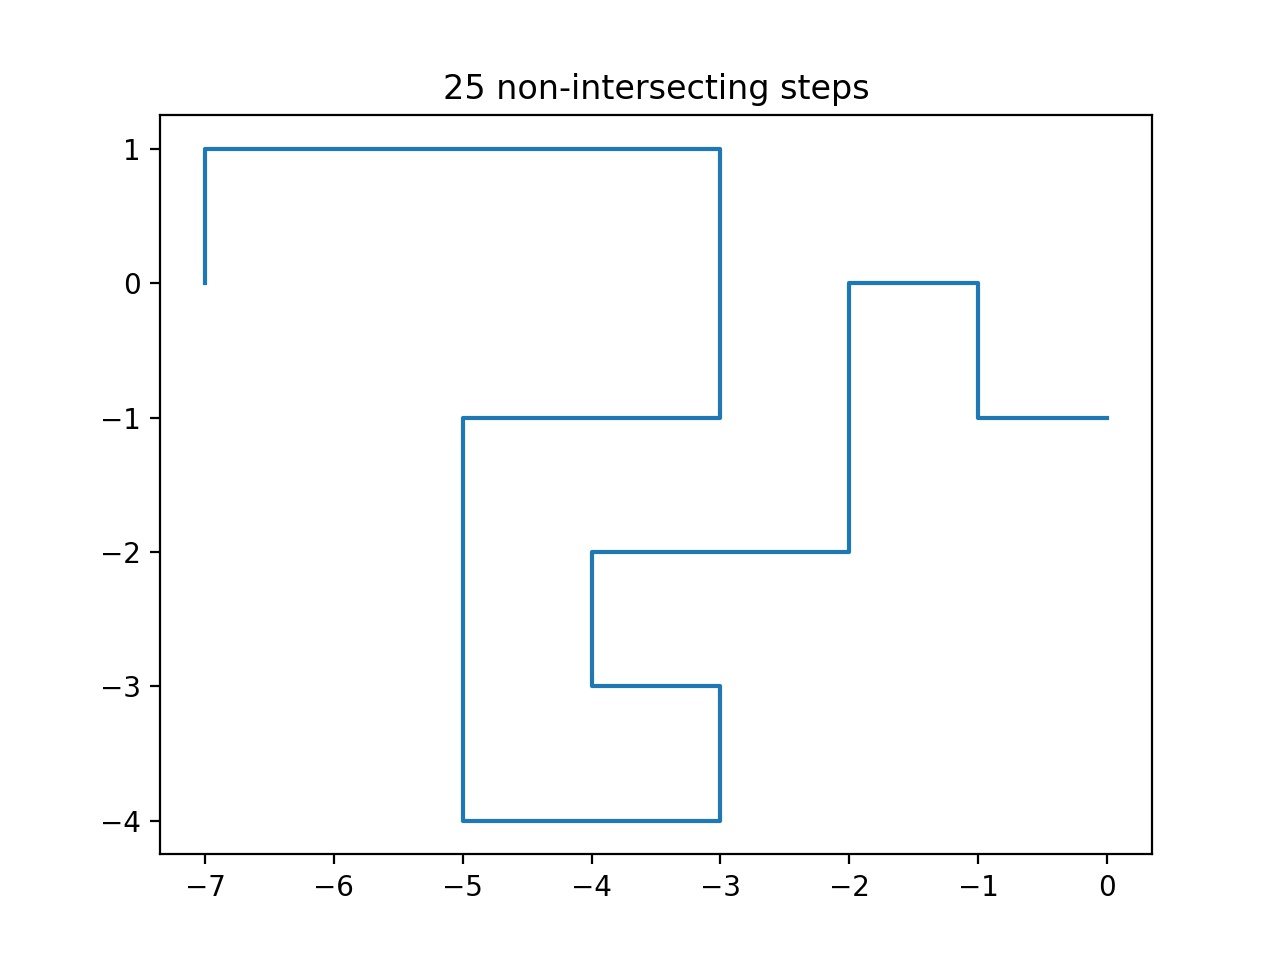
\includegraphics[ width=0.33\textwidth]{25.jpg}}
   \subfloat[\label{mt-simtask}]{%
      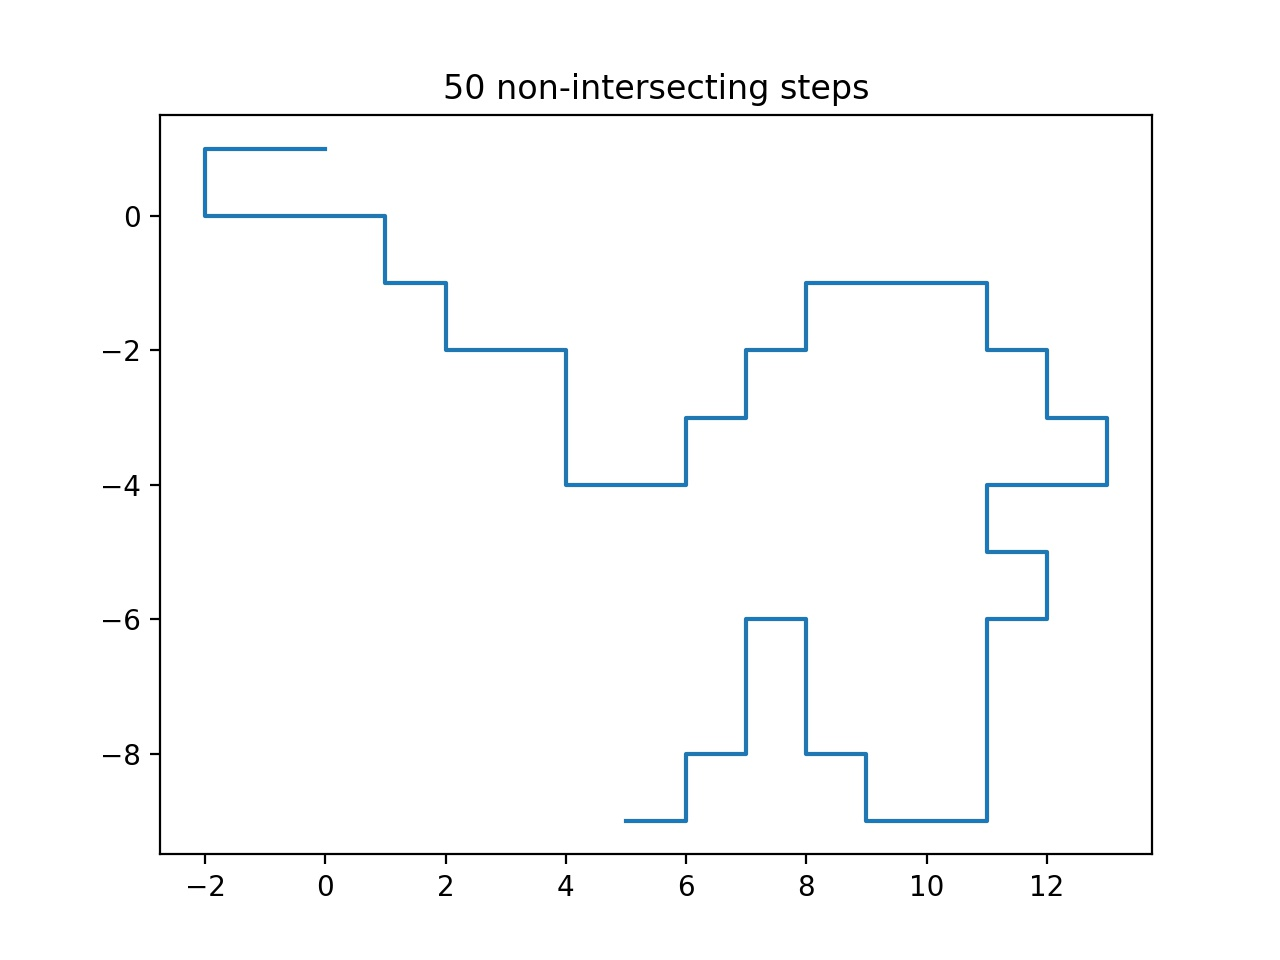
\includegraphics[ width=0.33\textwidth]{50.jpg}}\\
   \caption{\label{workflow} (a) 5 steps (b) 25 steps (c) 50 steps}
\end{center}
\end{figure*}

\noindent The non-intersecting walks were generated by 
by storing all previously visited sites of the same walk and terminating when a previously visited
is revisited. For the improved variant, moves are generated  in three directions, and not back in the previous direction. For 50 steps, the improved variant was utilized.
\subsubsection*{Comparison between original and improved variant}
\begin{figure*}[ht!]
\begin{center}
   \subfloat[\label{genworkflow}]{%
      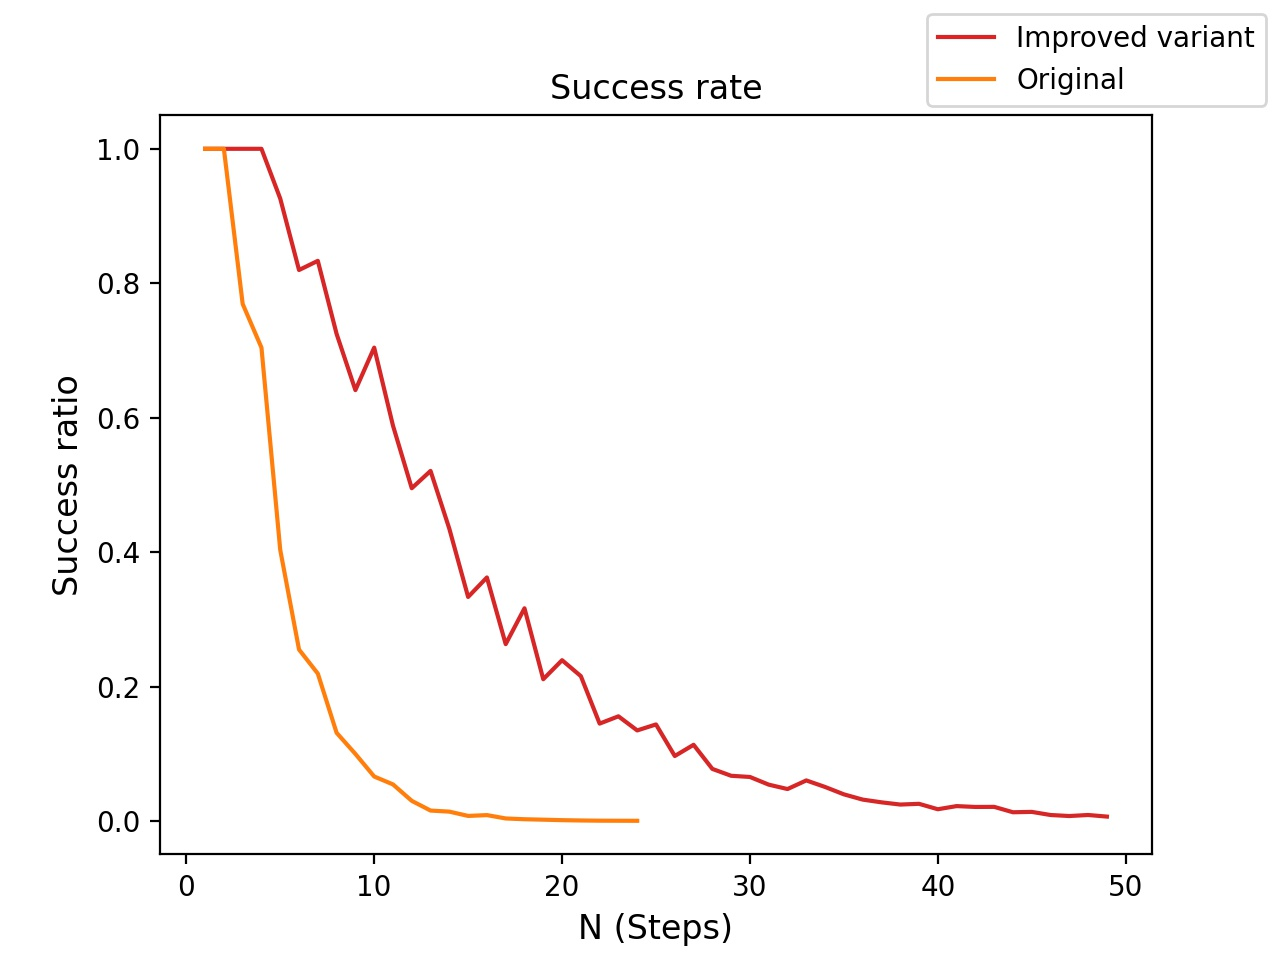
\includegraphics[width=0.4\textwidth]{Success.jpg}}
   \subfloat[\label{pyramidprocess}]{%
      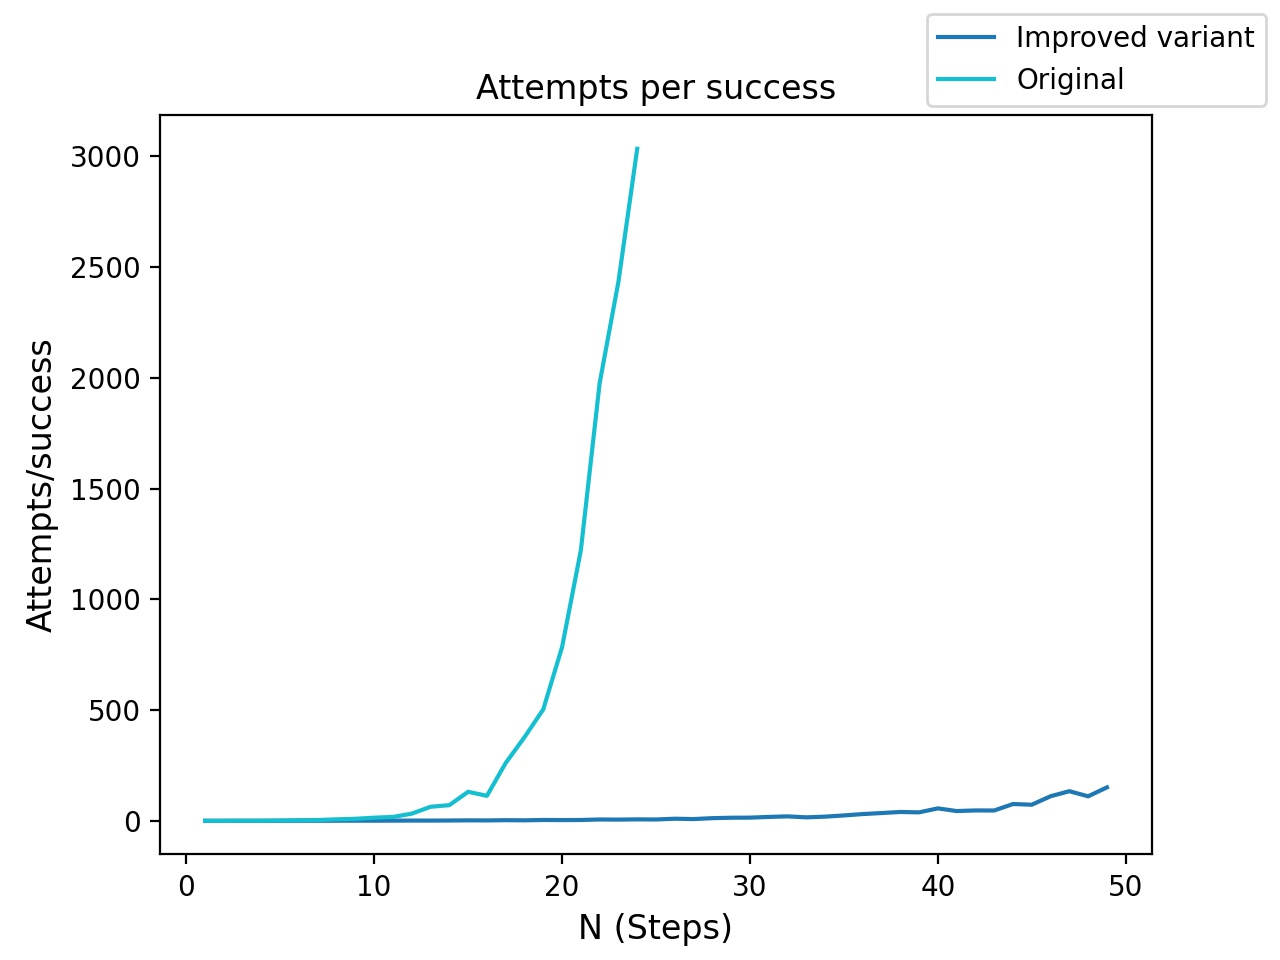
\includegraphics[ width=0.4\textwidth]{Attempts.jpg}}\\
   \caption{\label{workflow} (a) Success rate (b) Attempts per success}
\end{center}
\end{figure*}
\noindent For the original variant, the attempts per success ratio increases exponentially and as
\newline $N \to 30$, the number of attempts starts diverging. It can therefore be concluded that this variant is not suitable for $N > 30$ and \textit{unable} to generate the random walk for $N = 50$.

\newpage
\noindent For the improved variant, a substantially greater amount of steps can be utilized and for $N \leq 3$, a $100 \%$ success rate is to be observed. 
Also, note the success rate for 20 steps in the original variant correlates to that of 50 steps in the enhanced one, which is a considerable improvement.

\subsection*{2.1e) Distance comparison - intersecting and non-intersecting walks}

\begin{figure*}[ht!]
\begin{center}
   \subfloat[\label{genworkflow}]{%
      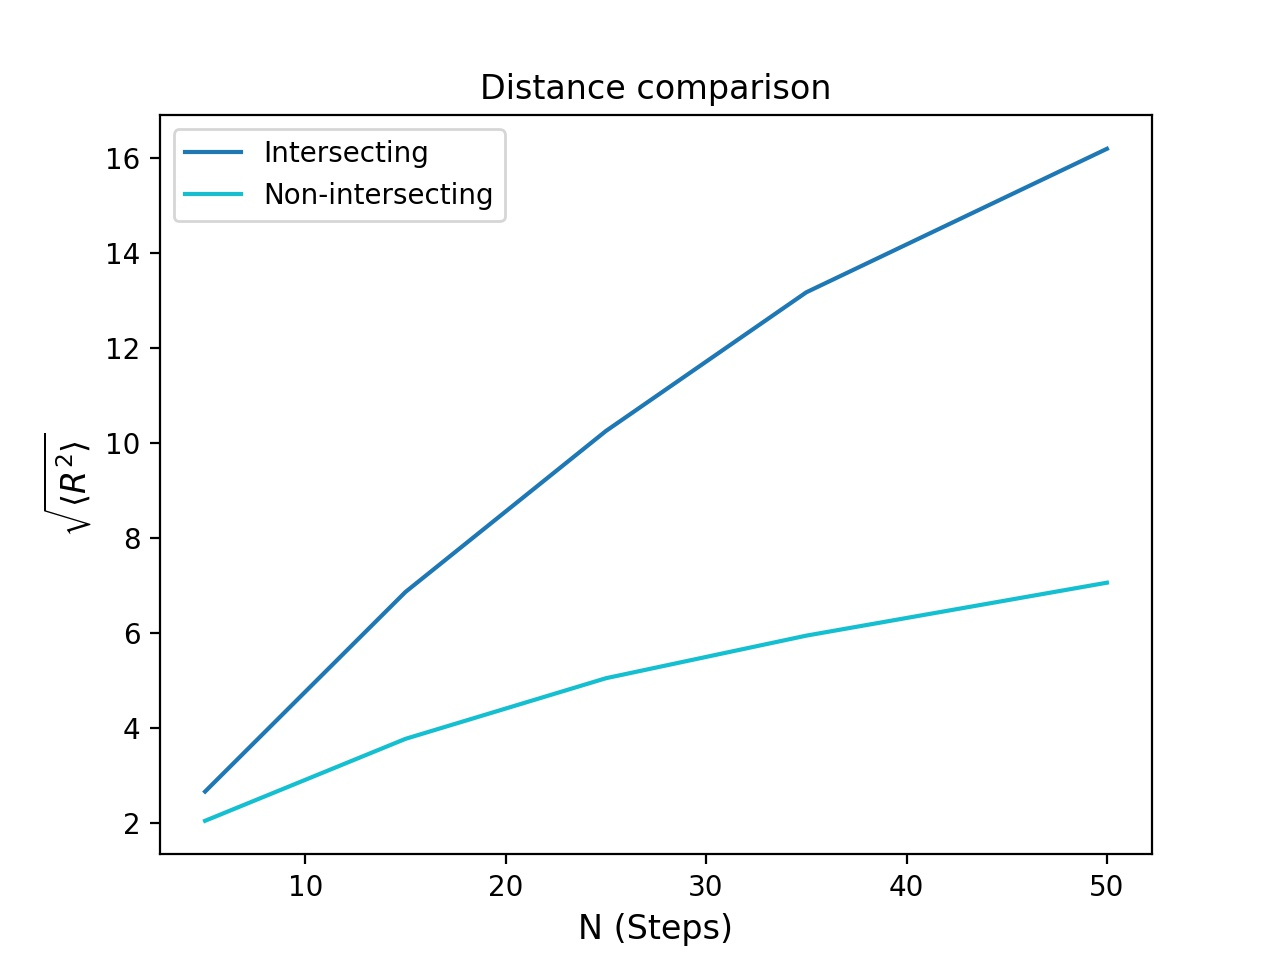
\includegraphics[width=0.45\textwidth]{Sqrt_distance.jpg}}
   \subfloat[\label{pyramidprocess}]{%
      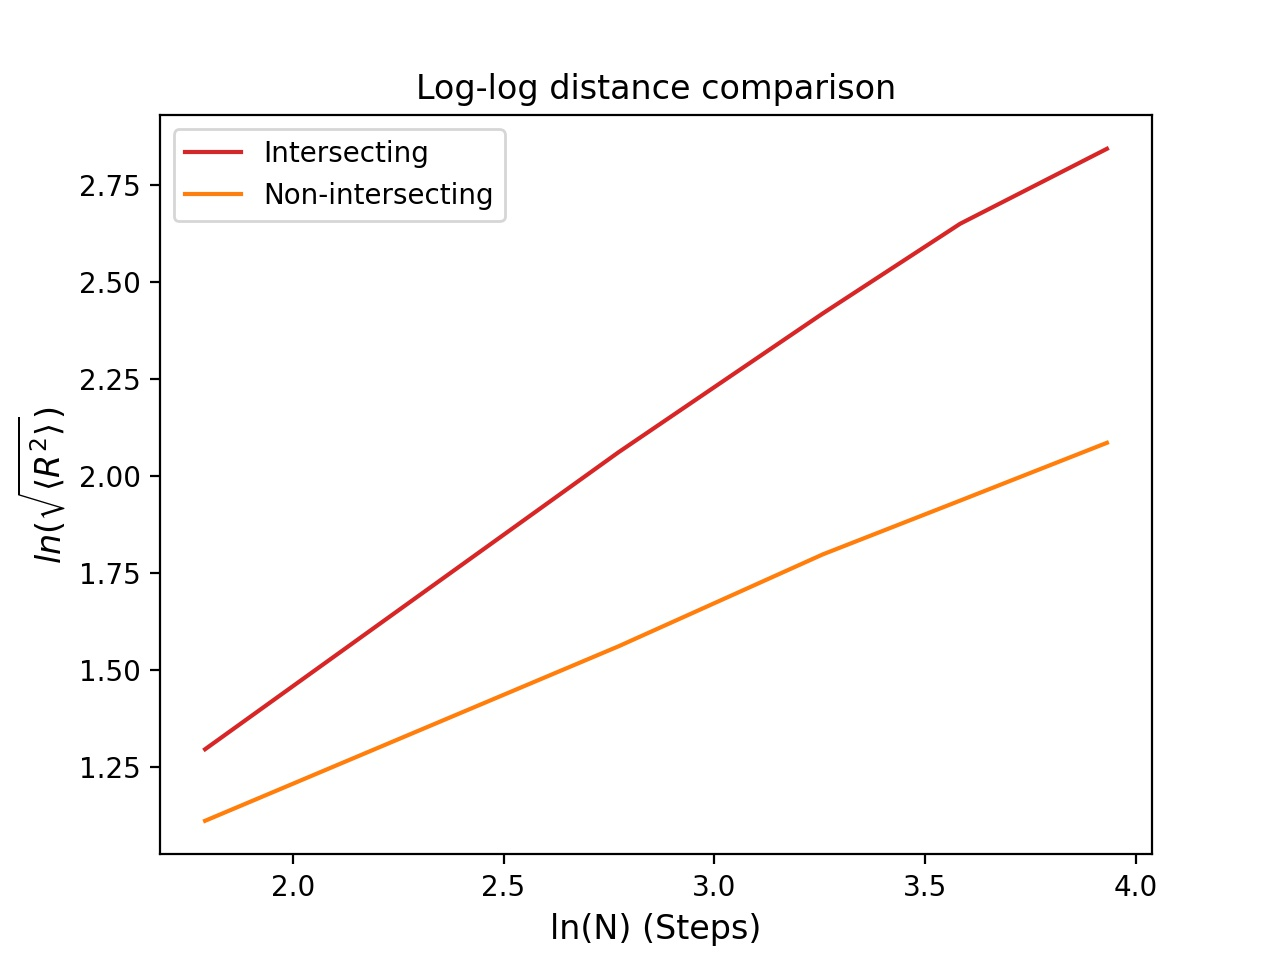
\includegraphics[ width=0.45\textwidth]{Log_distance.jpg}}\\
   \caption{\label{workflow} (a) Distance comparison  (b) Log-log distance  comparison}
\end{center}
\end{figure*}



\noindent As can be noted, the intersecting walks traverse longer distances than their non-intersecting counterparts. It can also be concluded that the the distances (mean square end-to-end) for intersecting walks follow a slightly polynomial relationship while the the distances in non-intersecting walks correlate linearly. 

\newpage
\section*{Project 2.2}
\subsection*{2.2a) Cellular automaton traffic model}
The traffic model was simulated with 10 cars at each respective position, road length $L = 50$, maximum speed $v_{max} = 2$ and speed reduction probability $p = 0.5$. In total, 1000 simulations are executed for each car for 100 time steps. 
Each car density $N_{cars}/L$ is computed with car numbers according to
\begin{equation*}
N_{cars} \in \{ 0, 2, 5, 7, 10, 15, 20, 25, 30, 35, 40, 45, 50 \}
\end{equation*}
For the fundamental diagram, the flow rate is determined according to $\Sigma v_{cars}/L$ and plotted against the car densities.
\begin{figure*}[ht!]
\begin{center}
   \subfloat[\label{genworkflow}]{%
      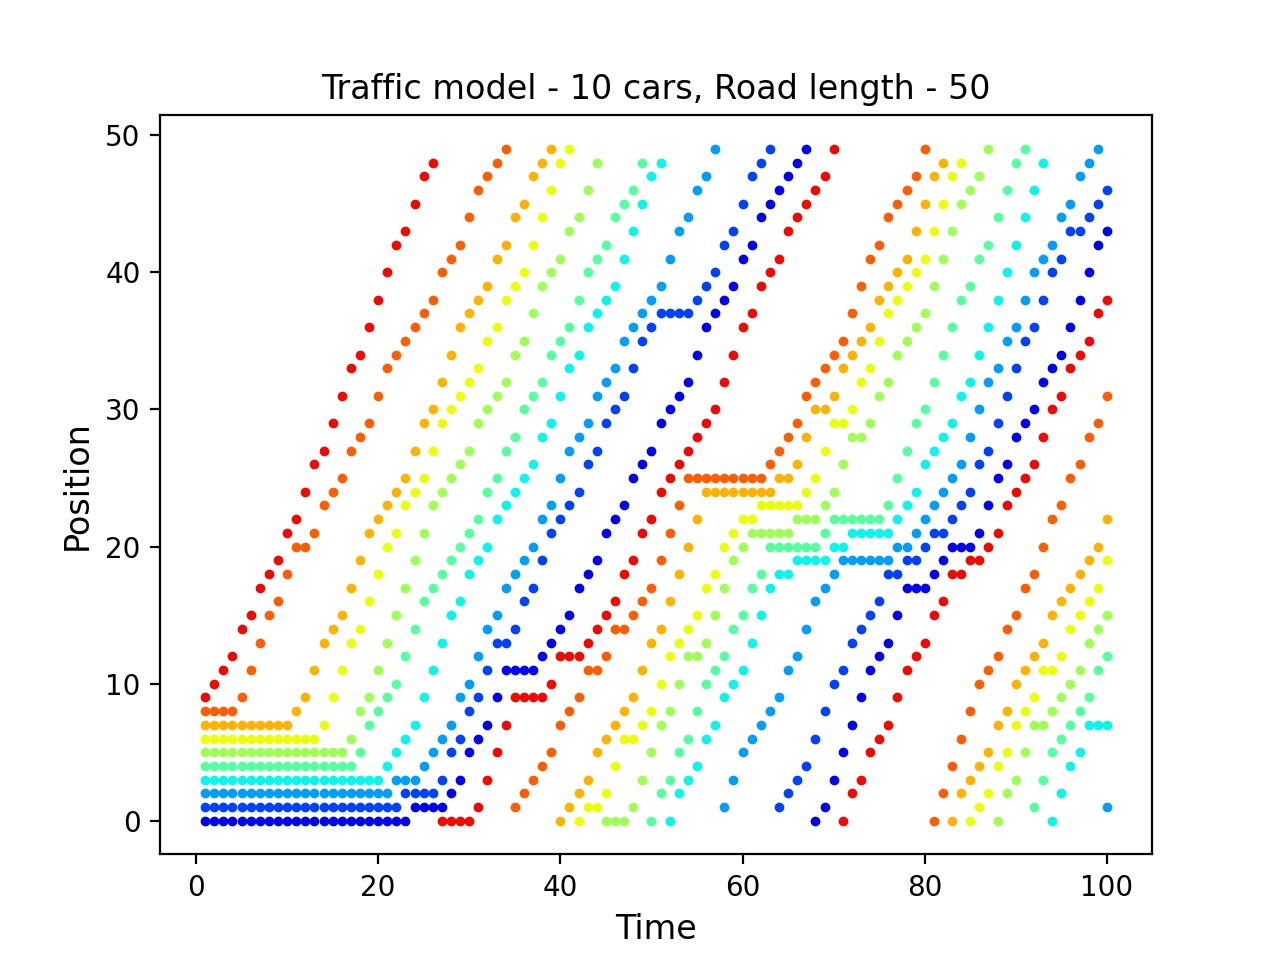
\includegraphics[width=0.45\textwidth]{Traffic_simulation.jpg}}
   \subfloat[\label{pyramidprocess}]{%
      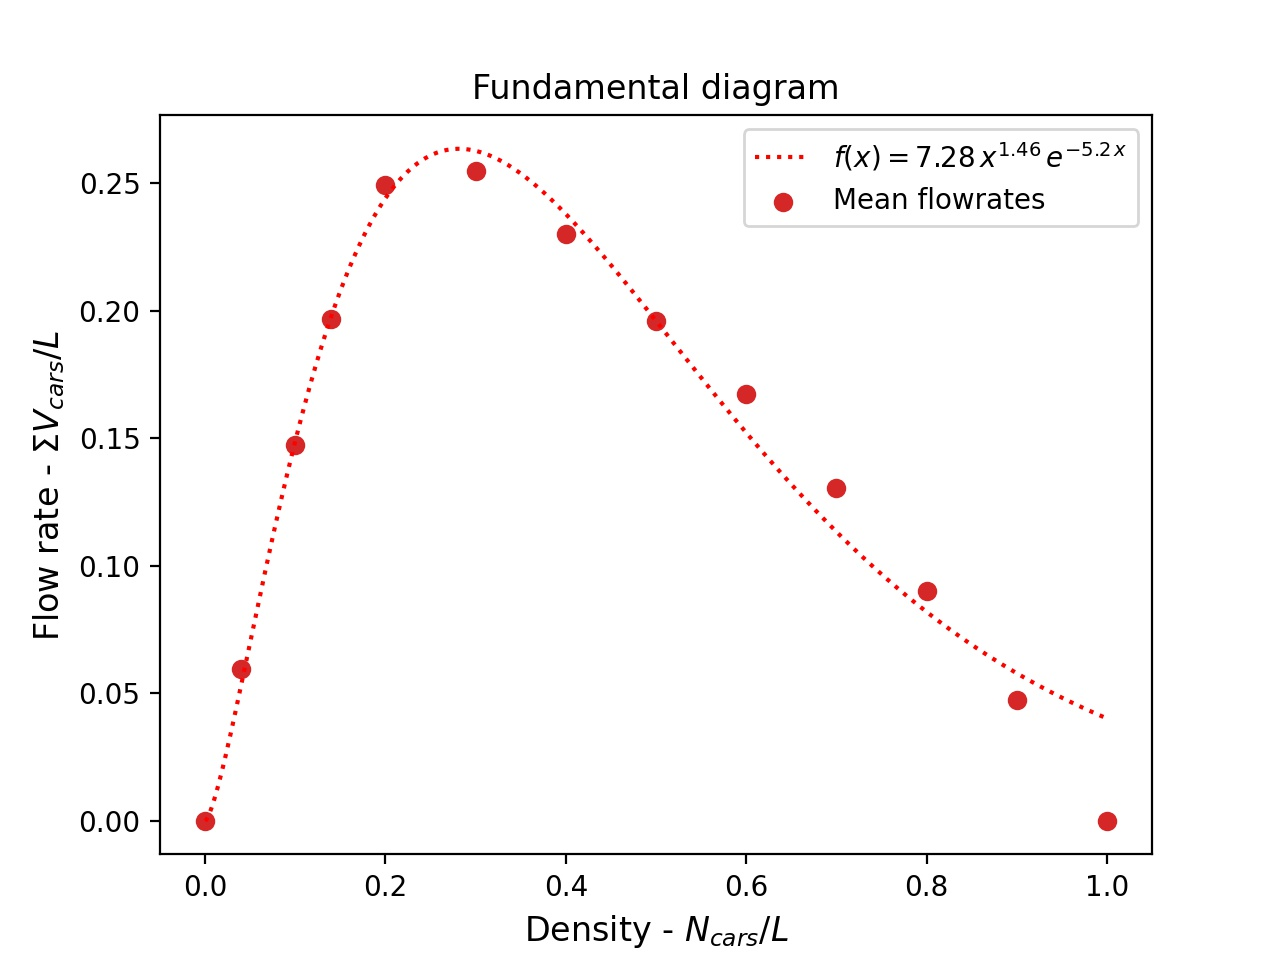
\includegraphics[ width=0.45\textwidth]{Fundamental_diagram.jpg}}\\
   \caption{\label{workflow} (a) Traffic simulation (b) Fundamental diagram}
\end{center}
\end{figure*}

\noindent As can be noted, the qualitative shape of the fundamental diagram follows the exponential relation of 
\begin{equation*}
f(x) = cx^k e^{-ax} = 7.28x^{1.46} e^{-5.2x}
\implies f(d) \approx 7.3\sqrt{d^3} e^{-5.2d}
\end{equation*}
This function has been regressed \footnote{Least square regression} according to the mean flow rates data points and shown in the fundamental diagram in Figure 11. At a density of 0.3, the maximum flow rate attained, while reducing and plateauing as it approaches a value of 1. To clarify, traffic jams will begin occurring at a car density of 0.3.

\newpage
\subsection*{2.2b) Statistical accuracy}
The statistical accuracy can be interpreted as the standard error of the flow rates for multiple simulations. With L = 50, 25 cars, $v_{max} = 2$, $p = 0.5$ and 100 time steps, the standard errors have been computed plotted in the figure below.
\begin{figure*}[ht!]
\begin{center}
    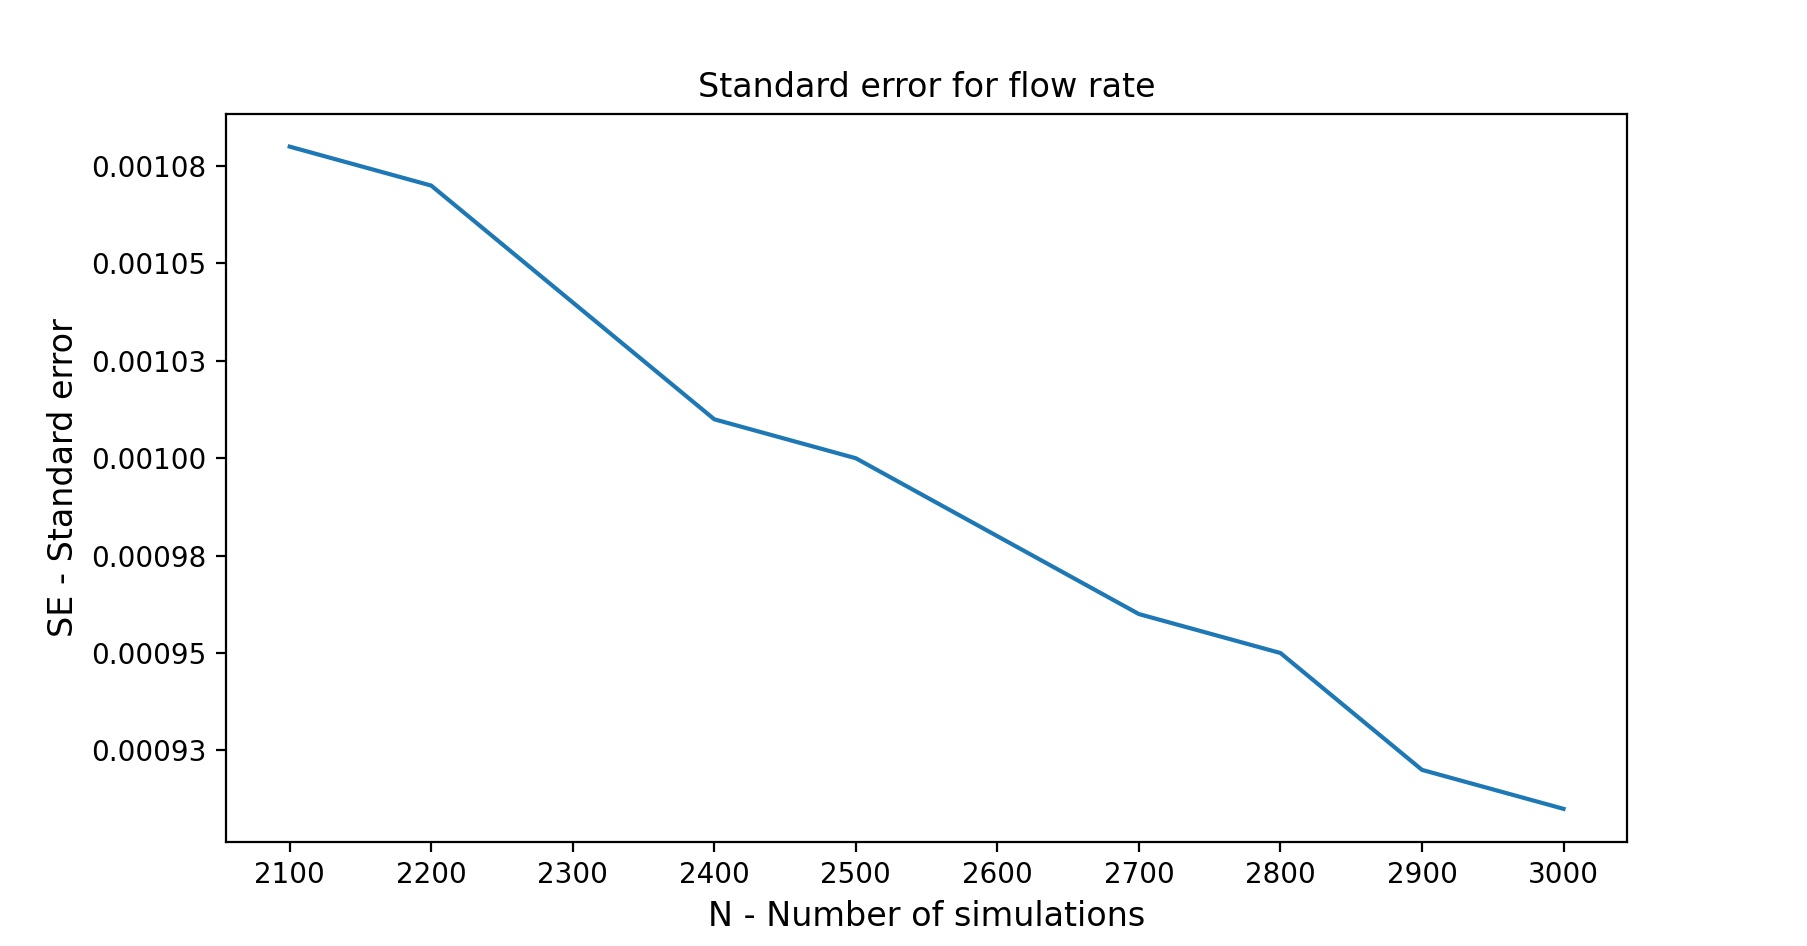
\includegraphics[width=0.6\textwidth]{Standard_error.jpg}
 \caption{}
\end{center}
\end{figure*}

\noindent As can be noted, the standard error approaches 0.001 within a range of 2500 simulations, with the dependence on equilibration time only being marginal. This can be attributed to the fact that the flowrates tend to equilibrate at equivalent values for car densities regardless of initial conditions.

\subsection*{2.2c) Dependence on road length}
With the same parameters and car densities as in 2.2a), the variation in road length values as in $L \in \{5, 10, 25, 50, 75, 100, 150\}$,
yields the following juxtaposed diagram.
\begin{figure*}[ht!]
\begin{center}
    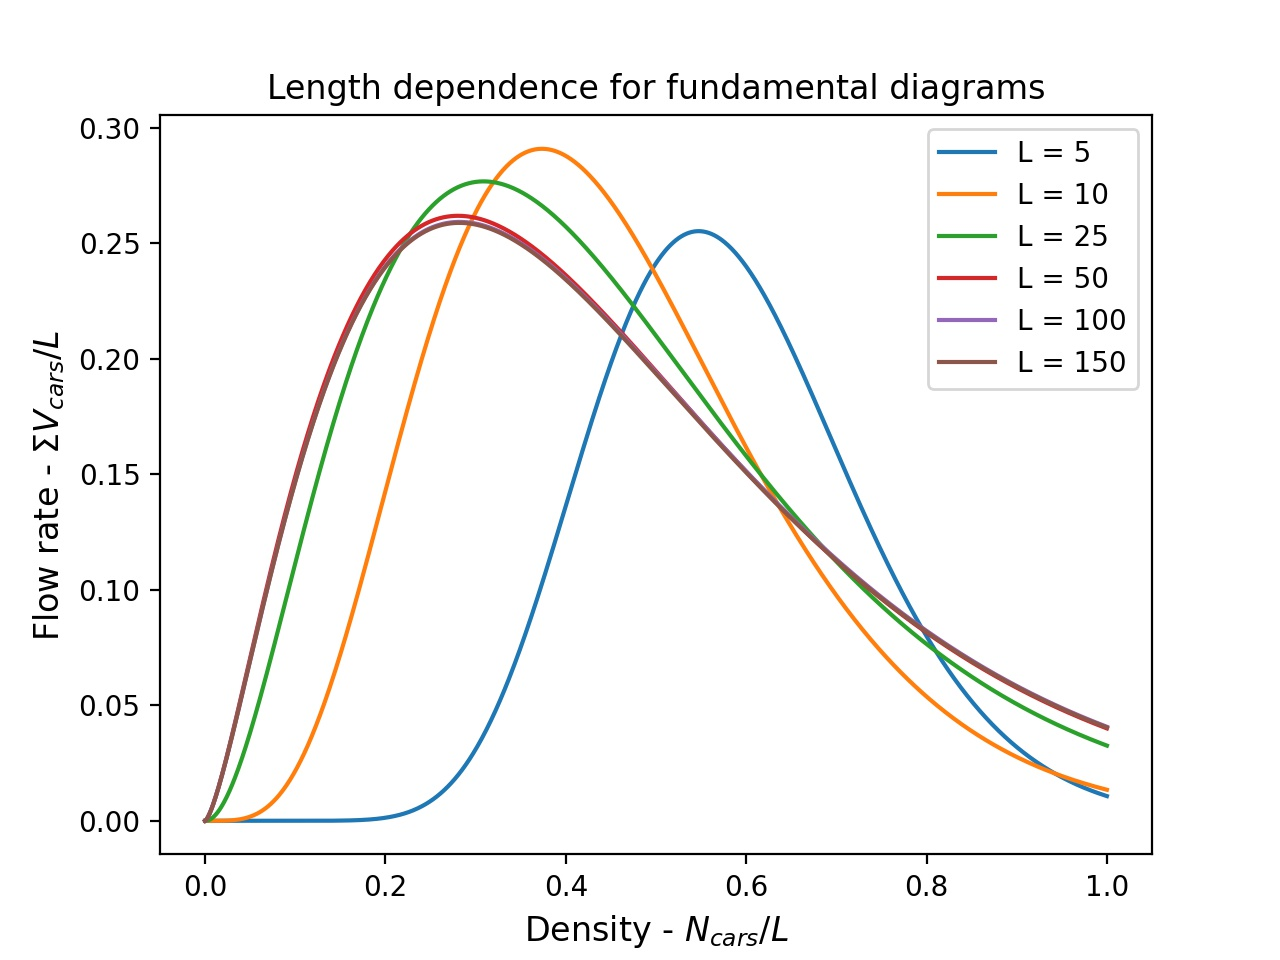
\includegraphics[width=0.47\textwidth]{Length_dependence.jpg}
 \caption{}
\end{center}
\end{figure*}

\noindent As in the previous case, the flow rate data points have also been regressed with the same exponential function. 
\newpage
\noindent An apparent dependence on road length is to be noted for road length L $<$ 50. 
For L $\geq$ 50, the fundamental diagrams start stabilizing and a change in L affects the results minusculely.
This can also be attributed to the rationality in utilizing L = 50 has for all previous simulations, as greater road lengths require significantly longer equilibration times.

\subsection*{2.2d) Dependence on maximum velocity}
Utilizing the same parameters and course of action as in 2.2a), but varying $v_{max}$ according to 
$v_{max} \in \{1, 2, 5\}$, the following traffic simulations and fundamental diagrams were yielded.
\begin{figure*}[ht!]
\subsubsection*{Traffic simulations}
\begin{center}
   \subfloat[\label{genworkflow}]{%
      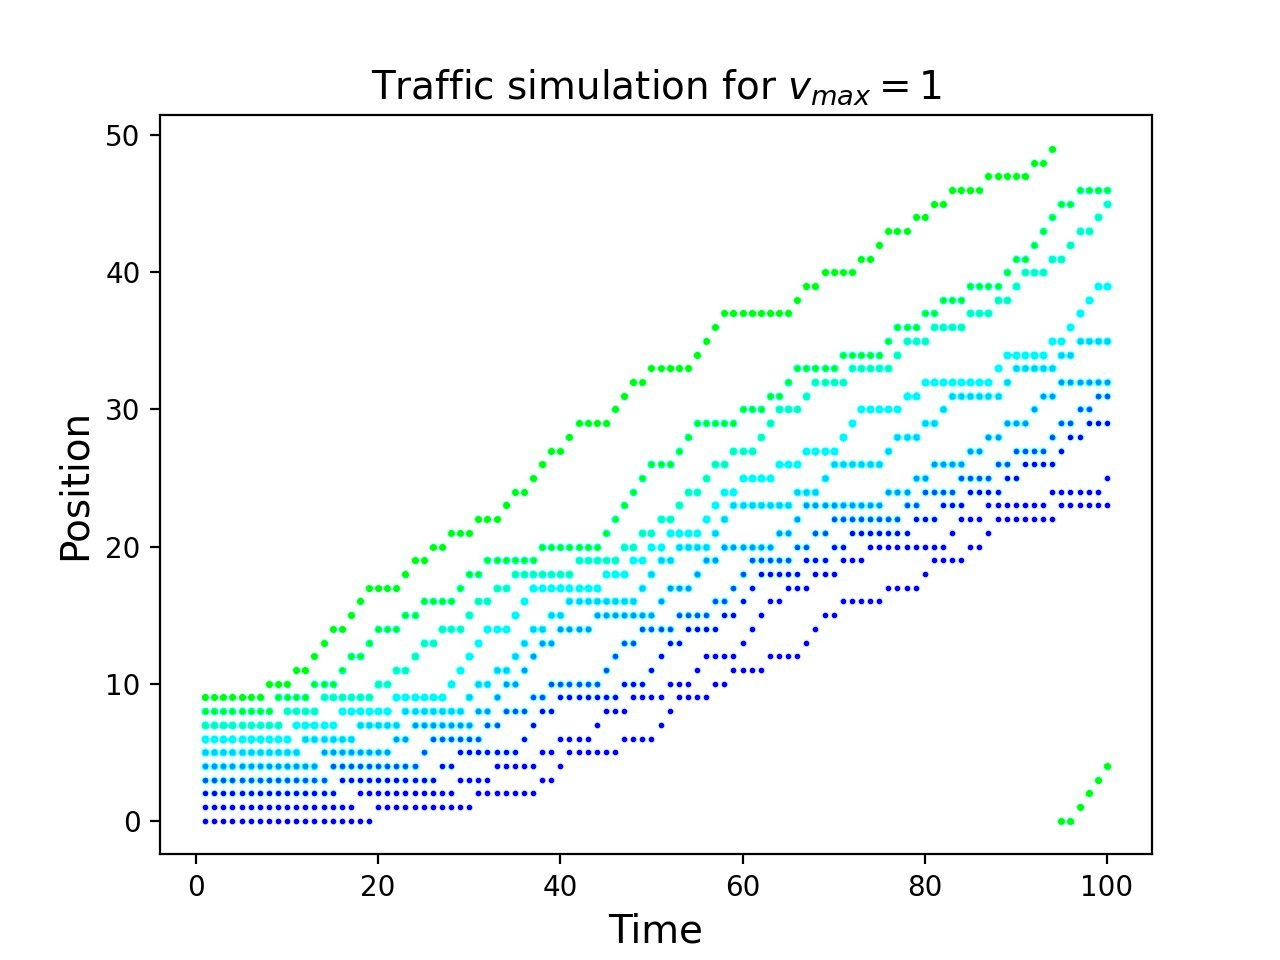
\includegraphics[width=0.33\textwidth]{Traffic_vmax=1.jpg}}
   \subfloat[\label{pyramidprocess}]{%
      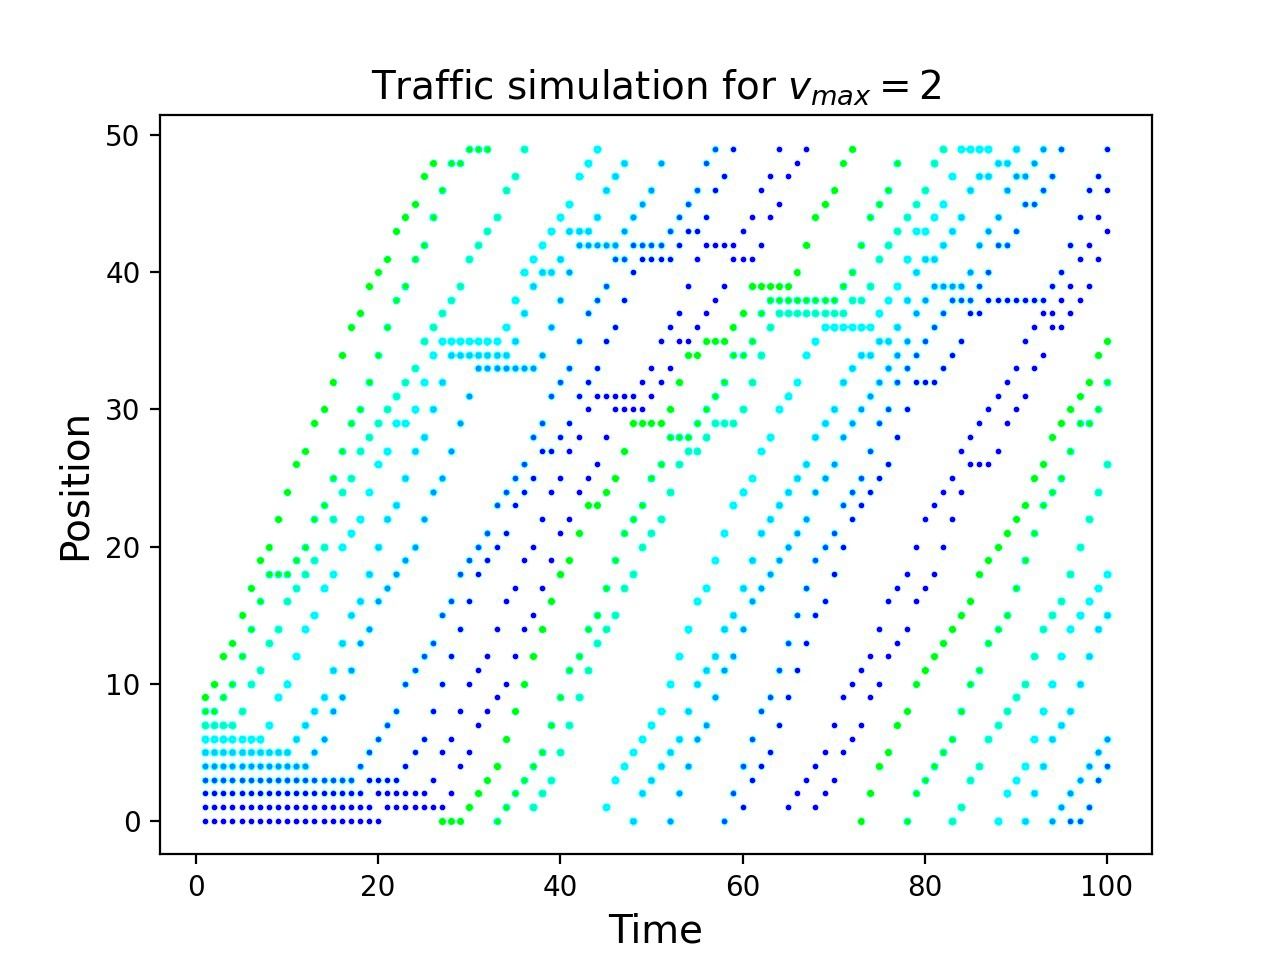
\includegraphics[ width=0.33\textwidth]{Traffic_vmax=2.jpg}}
   \subfloat[\label{mt-simtask}]{%
      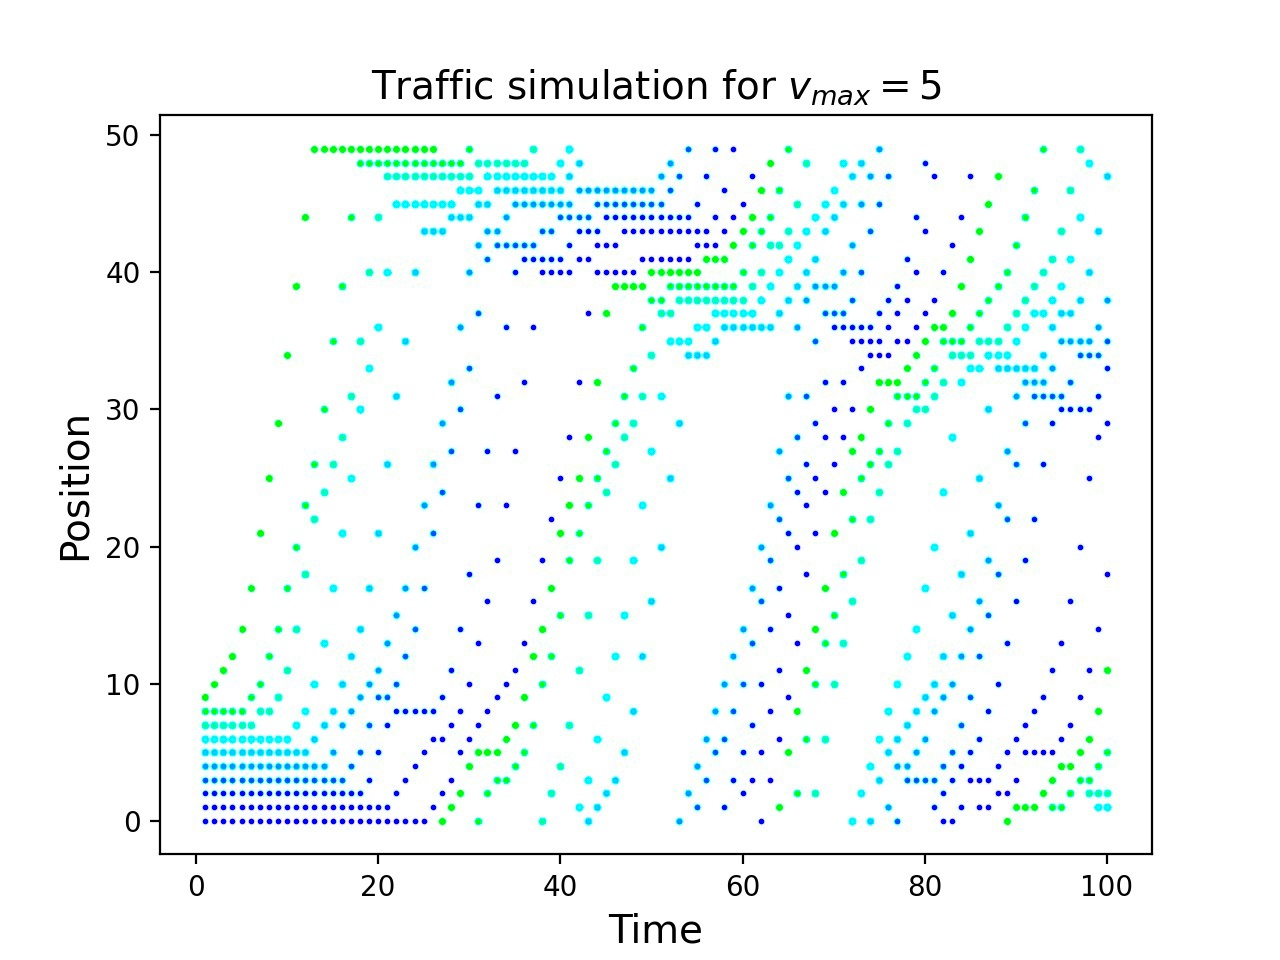
\includegraphics[ width=0.33\textwidth]{Traffic_vmax=5.jpg}}\\
   \caption{\label{workflow} (a) $v_{max}=1$ (b) $v_{max}=2$ (c) $v_{max}=5$}
\end{center}
\end{figure*}

\begin{figure*}[ht!]
\subsubsection*{Fundamental diagrams}
\begin{center}
    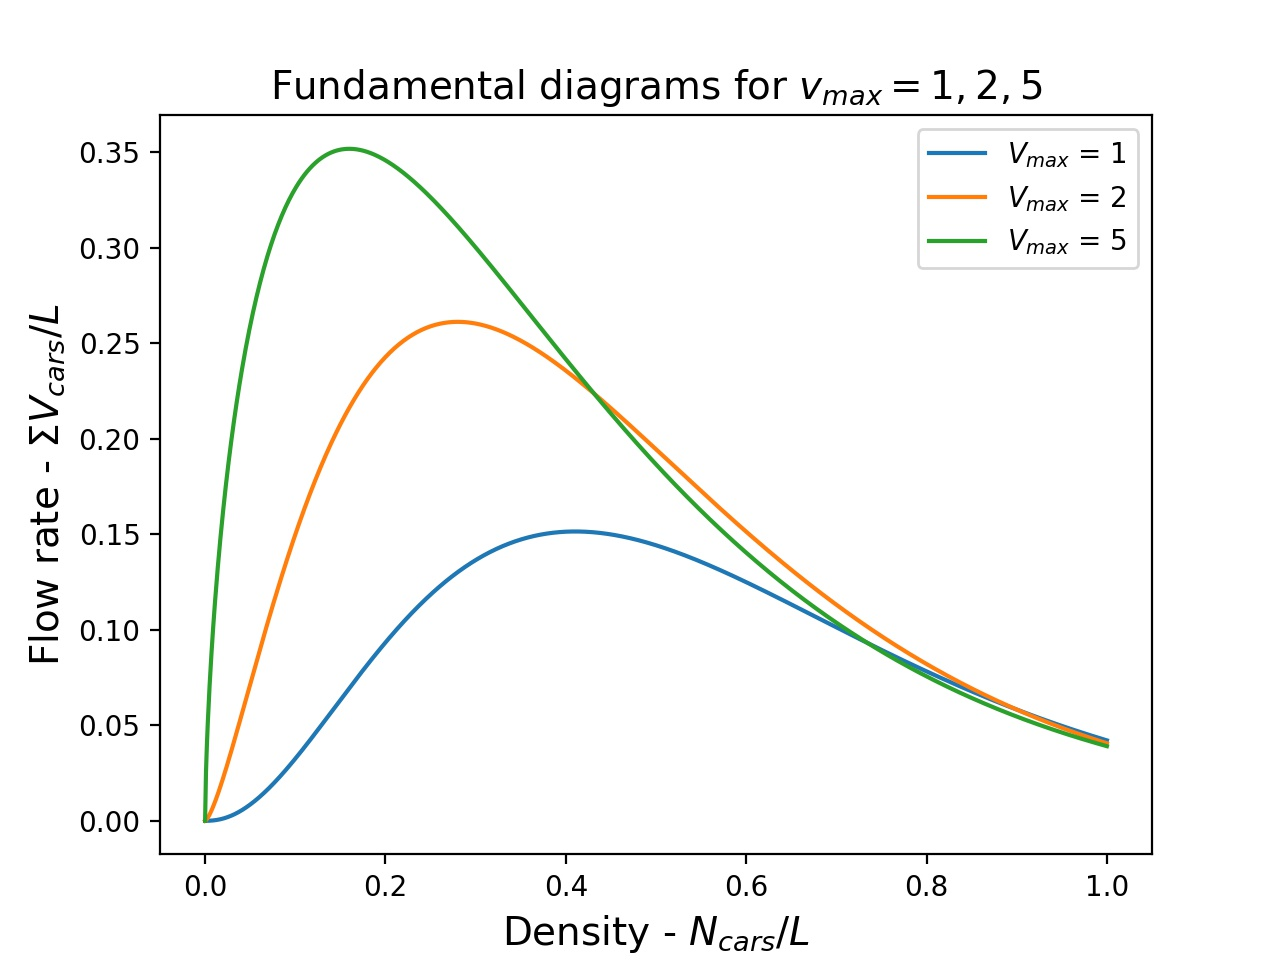
\includegraphics[width=0.44\textwidth]{Velocity_comparison.jpg}
 \caption{Fundamental diagrams for $v_{max}$ = 1, 2, 5}
\end{center}
\end{figure*}

\noindent As can be noted, an increase of $v_{max}$ decreases the density required to attain the maximum flow rate. Thus, traffic jams will occur more frequently. An increase of $v_{max}$ also results in greater flow rates for all densities. As a result, at greater maximum velocities the frequency for traffic jams will increase but they will resolve earlier due to the streamlined flow rates.
\newpage



\subsection*{2.2e) Dependence on speed reduction probability}
Utilizing the same parameters and course of action as in 2.2a), but varying $p$ according to 
$p \in \{0.2, 0.5, 0.8\}$, the following traffic simulations and fundamental diagrams were yielded.
\begin{figure*}[ht!]
\subsubsection*{Traffic simulations}
\begin{center}
   \subfloat[\label{genworkflow}]{%
      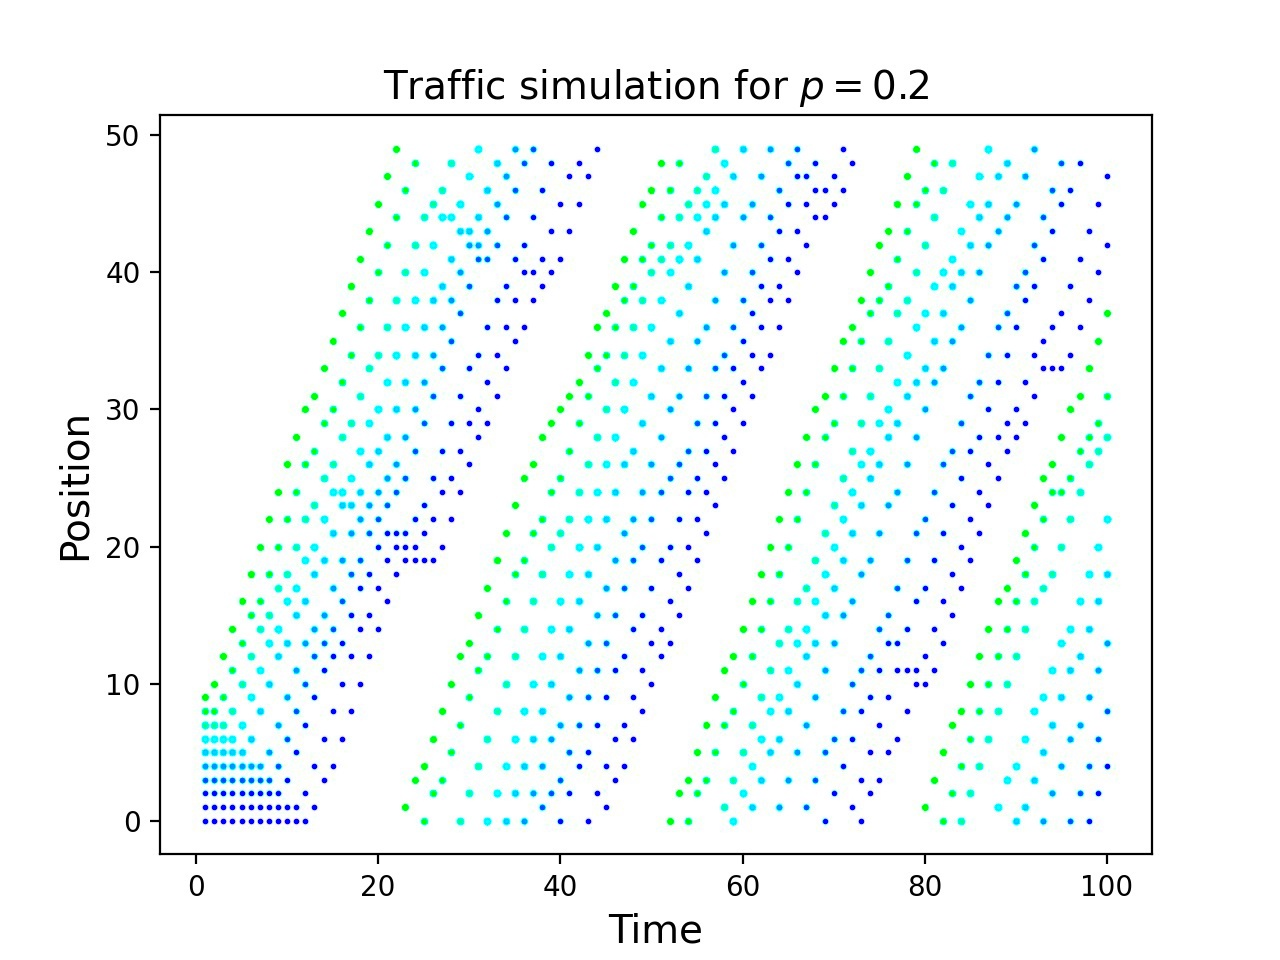
\includegraphics[width=0.33\textwidth]{Traffic_p=0.2.jpg}}
   \subfloat[\label{pyramidprocess}]{%
      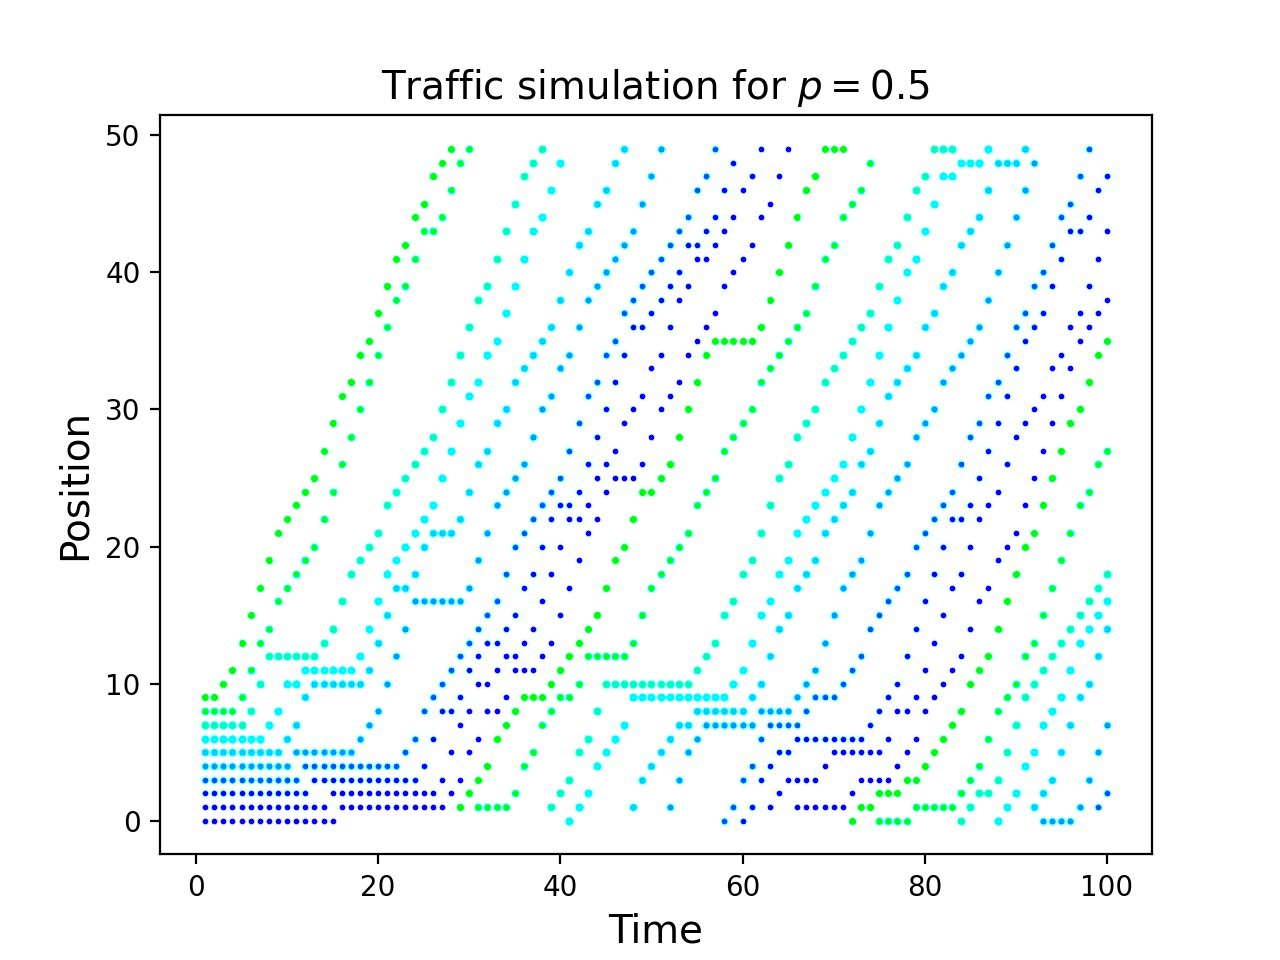
\includegraphics[ width=0.33\textwidth]{Traffic_p=0.5.jpg}}
   \subfloat[\label{mt-simtask}]{%
      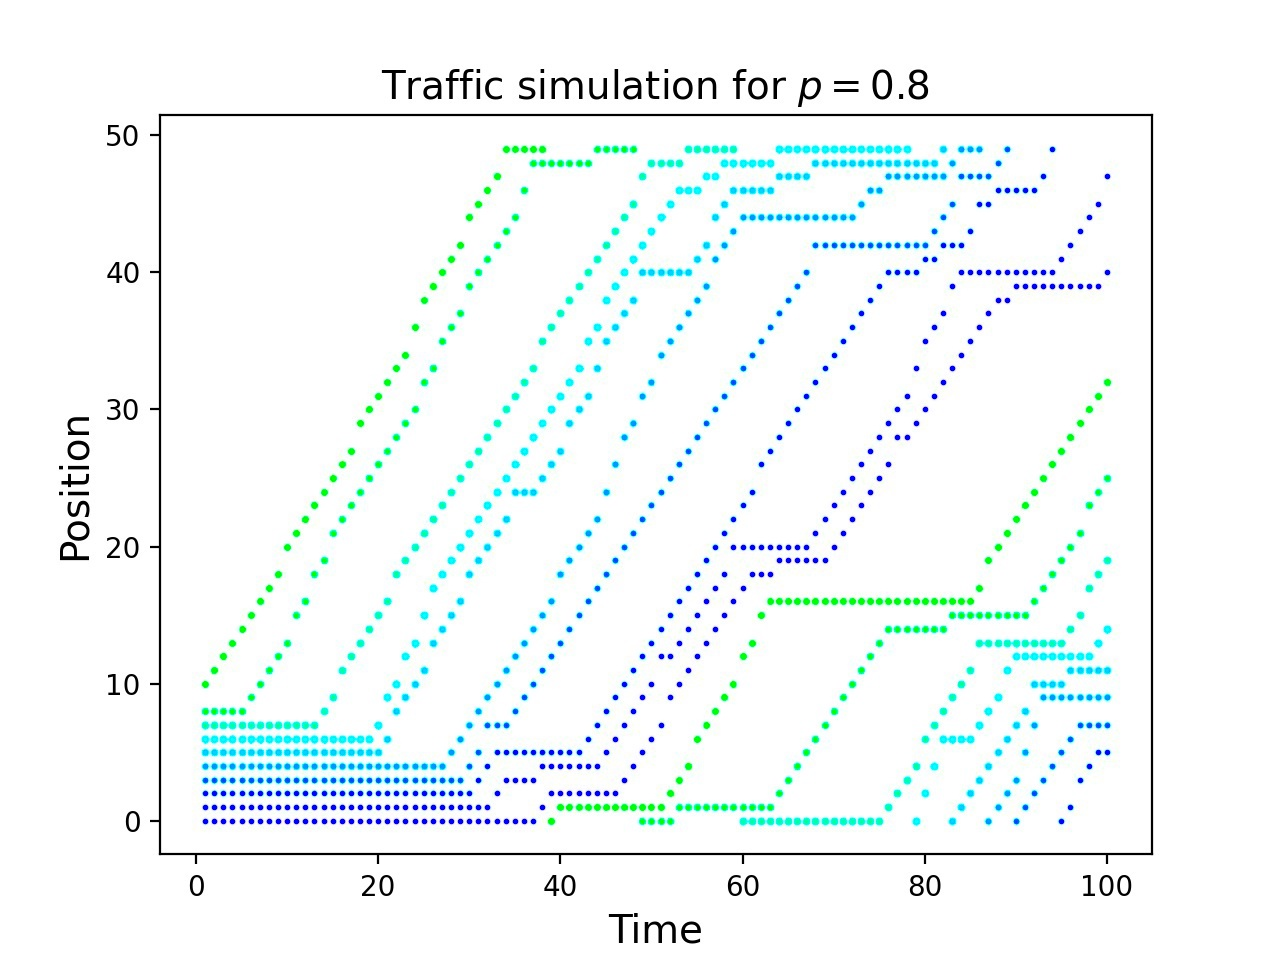
\includegraphics[ width=0.33\textwidth]{Traffic_p=0.8.jpg}}\\
   \caption{\label{workflow} (a) $p=0.2$ (b) $p=0.5$ (c) $p=0.8$}
\end{center}
\end{figure*}

\begin{figure*}[ht!]
\subsubsection*{Fundamental diagrams}
\begin{center}
    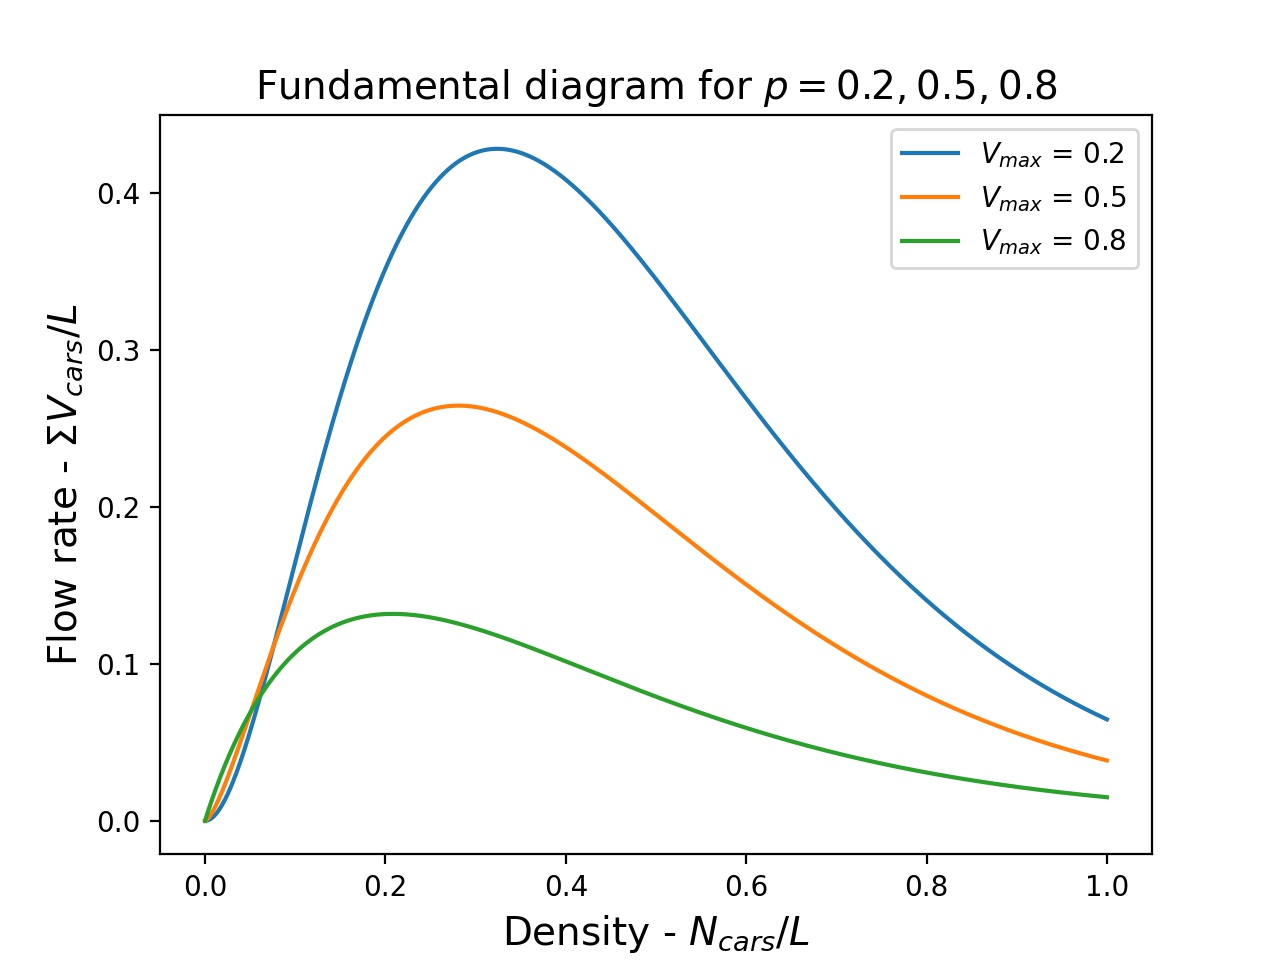
\includegraphics[width=0.44\textwidth]{Probability_comparison.jpg}
 \caption{Fundamental diagrams for p = 0.2, 0.5, 0.8}
\end{center}
\end{figure*}

\noindent As can be noted, an increase of speed reduction probability (braking) decreases the density required to attain the maximum flow rate. However, this effect is more marginal compared to the increase of maximum velocity. An increase of speed reduction probability also decreases the flow rates for all densities. Thus, the size, frequency and propagation of traffic jams will increase the more likely drivers are to braking.
\end{document}
